\documentclass[twoside]{article}
%------------------------------PAQUETES------------------------------
\usepackage{booktabs}
\usepackage[usenames,dvipsnames,svgnames,table]{xcolor}
\usepackage[utf8]{inputenc}
\usepackage{amsmath}
\usepackage{graphicx} % Required for inserting images
\usepackage[spanish]{babel} %diccionario
\usepackage{subfigure}     %divide figuras en subfiguras y las etiqueta individualmente
\usepackage{graphicx}   %incluye imágenes
%\usepackage[usenames]{color}    %se usa nombres en colores en vez de códigos RGB [alternativa]
\usepackage{subcaption}     %subtitulo de tablas y figuras
\usepackage{vmargin}    %ajusta los márgenes verticales del documento
\usepackage{fancyhdr}   %personaliza el encabezado y píe de página del documento
\usepackage{enumerate}  %controla el formato de listas enumeradas
\usepackage{hyperref}   %crea hipervínculos en el documento como links de páginas web
\usepackage{float}  %da control sobre elementos flotantes como figuras o tablas
\usepackage{soulutf8}   %resalta o tacha textos con distintos estilos
\usepackage{xcolor} %ofrece opciones más avanzadas que [usename][color]
\usepackage{soul} %subraya palabras


%------------------------------ESTILO DE LENGUAJE DE PROGRAMACIÓN------------------------------
%estructura para ingresar código
\usepackage{color} %paquete de color personalizado
\usepackage{listings} %formatea y muestra código fuente
\definecolor{codegreen}{rgb}{0,0.6,0} 
\definecolor{codegray}{rgb}{0.5,0.5,0.5}
\definecolor{codepurple}{rgb}{0.58,0,0.82}
\definecolor{backcolour}{rgb}{0.95,0.95,0.92}

\lstdefinestyle{mystyle}{                   %define un nuevo estilo para listados de código
    backgroundcolor=\color{backcolour},     %color de fondo
    commentstyle=\color{codegreen},         %color de los comentarios
    keywordstyle=\color{magenta},           %color de palabras claves
    numberstyle=\tiny\color{codegray},      %estilo de los números en linea
    stringstyle=\color{codepurple},         %color para las cadenas de  texto
    basicstyle=\ttfamily\footnotesize,      %tipo de letra y tamaño para todo el código
    breakatwhitespace=false,                %false = desactiva saltos de linea automático en el cuerpo del código
    breaklines=true,                        %true = permite salto de línea automático al final del código
    captionpos=b,                           %agrega leyenda del listado de código en la parte inferior
    keepspaces=true,                        %preserva los espacios en blanco dentro del código
    numbers=left,                           %muestra los números de línea a la izquierda del código
    numbersep=5pt,                          %espacio de separación entre números de línea y código
    showspaces=false,                       %false = oculta los espacios en blanco.
    showstringspaces=false,                 %false = oculta los espacios dentro de la cadena de texto
    showtabs=false,                         %false = no muestra tabuladores con carácteres especiales
    tabsize=2                               %define el número de espacios para un tabulador de código
}

\lstset{style=mystyle}      %establece el estilo configurado por defecto.

%-----------------------------ENCABEZADO Y PÍE DE PÁGINA-----------------------------
% Definir estilo fancy
\fancyhf{}  %limpia o borra el formato anterior del encabezado y pie de págica
%-----------------ENCABEZADO-----------------
\fancyhead[RE]{\nouppercase{\rightmark}}  
\fancyhead[LO]{\nouppercase{\leftmark}} 
\fancyhead[RO]{\thepage}    
\fancyhead[LE]{\thepage}

%-----------------------------FORMATO DE PÁGINA-----------------------------
% Definir formato de página
\setpapersize{A4}        % tipo de página
\setmargins{2.5cm}       % margen izquierdo
{1.5cm}                  % margen superior
{16cm}                   % anchura del texto
{23.42cm}                % altura del texto
{10pt}                   % altura de los encabezados
{1cm}                    % espacio entre el texto y los encabezados
{0pt}                    % altura del pie de página
{2cm}                    % espacio entre el texto y el pie de página
\headheight=12pt    

% ---------------------------------INICIO DEL DOCUMENTO---------------------------------

\begin{document}
%-----------------CARATULA-----------------
\begin{titlepage}
	\centering
    
\includegraphics[scale=0.3]{escudo-unvime.png}\par
    \vspace{1cm}
    {\bfseries\LARGE Universidad Nacional del Villa Mercedes \par}
    \vspace{1cm}
    {\scshape Escuela de Ingeniería y Ciencias Ambientales \par}
    {\scshape\Large Programador Universitario de Sistemas \par}
    \vspace{2cm}
    {\scshape\Huge Sistema de gestión de mercadería para quioscos minoristas \par}
    \vspace{1cm}
    {\itshape\Large Prática Profesional Supervisada \par}
	\vfill
	{\Large Autor: \par}
	{\Large Sombra Florencia \par}
	\vfill	
	{\Large Directores: \par}
	{\Large Mg. Gabriel Novillo Rangone \par}
	{\Large Ing. Alberto Ledesma \par}
\end{titlepage}

\newpage
\section*{Dedicatoria}
\textit{Gracias a mi madre y hermanos, que siempre me apoyaron}
\newpage
\tableofcontents
\newpage

\section{Introducción}
Los kioscos o comercios minoristas enfrentan desafíos particulares en la gestión de su mercadería, ya que reciben productos diariamente desde varios proveedores. En la mayoría de los casos, el manejo de stock y precios se realiza de forma manual, sin herramientas tecnológicas que permitan un control eficiente.\par
Esta situación \textbf{genera pérdidas económicas, errores de inventario y decisiones improvisadas que afectan tanto al comerciante como al cliente}, como la desorganización en el depósito, la falta de seguimiento de productos perecederos y la inexistencia de registros digitales, provoca que se desaproveche mercadería, se vendan productos vencidos o no se pueda responder rápidamente a las consultas de precio.\par
Dentro de estos comercios, \textbf{uno de los principales problemas} ocurre cuando el dueño o el empleado reciben muchos productos en el día y no actualizan los precios de todos ellos, produciendo situaciones donde se termina vendiendo un artículo con un precio no actualizado, uno asignado al azar para no hacer esperar al cliente, o directamente con un precio excesivo que espanta la venta, generando pérdidas económicas o la pérdida del cliente.\par
Frente a este escenario, se propone el \textbf{desarrollo de una aplicación web adaptada para celulares}, que permita a los kiosqueros contar con una herramienta accesible y confiable, que centralice toda la gestión de stock, los precios y los vencimientos en un sólo sistema.

\section{Planteo del problema}
Los principales problemas que enfrentan estos comercios son:
\begin{itemize}
    \item \textbf{La gestión manual de productos es ineficiente}, propensa a errores y genera pérdida de tiempo.
    \item \textbf{La vida útil de los productos perecederos no se gestiona adecuadamente}, generando pérdidas económicas o riesgos de salud.
    \item \textbf{La falta de visibilidad del stock}, esto impide detectar faltantes o tomar decisiones comerciales a tiempo.
    \item \textbf{No hay clasificación por lote ni por fecha de vencimiento}, lo que dificulta la rotación ordenada del inventario.
    \item \textbf{No se lleva un historial de ventas digital}, ni un análisis de rubros que permita anticipar la demanda.
    \item El sistema de precios es informal:
    \begin{itemize}
        \item \textbf{Se reciben productos y se calcula el precio de venta al día}, pero al pasar el tiempo, ese precio se va desactualizando.
        \item \textbf{Productos que no tienen precios, se coloca un precio 'al azar' o se basa en memoria}, esto causa pérdidas al comercio por vender demasiado barato o perder clientes por precios fuera del mercado.
    \end{itemize}
\end{itemize}
Estos problemas afectan la rentabilidad, reducen la eficiencia operativa y perjudican la experiencia del cliente.

\section{Solución propuesta}
Se propone desarrollar e implementar un sistema de gestión de productos especialmente diseñado para las necesidades de los kioscos minoristas, orientado a resolver los problemas mencionados mediante una plataforma accesible desde celulares, que combina tecnologías web con procesamiento mainframe.\par
El sistema se implementará en entorno LinuxONE, utilizando PHP para el desarrollo web y módulos escritos en COBOL para el procesamiento de datos críticos, garantizando rendimiento, escalabilidad y robustez.

Entre las funcionalidades claves del sistema, se destacan:
\begin{itemize}
    \item \textbf{Escaneo de productos desde la cámara del celular}: el sistema permite capturar el código de barras y obtener al instante el precio actualizado del producto.
    \item \textbf{Carga de precios desde boletas}: los precios podrán actualizarse de forma automática (OCR) o manual, a partir de las boletas de compra cargadas para el comerciante.
    \item \textbf{Ingreso por lotes y ubicación física}: los productos se clasifican por lote, rubro y ubicación dentro del depósito, mejorando el orden y la reposición.
    \item \textbf{Visualización del stock completo en tiempo real}, accesible desde cualquier dispositivo.
    \item \textbf{Sugerencia de promociones}: el sistema permitirá identificar rubros con vencimientos próximos y generar listas de ofertas por vencimientos, para evitar desperdicios.
    \item \textbf{Carga del precio sugerido por el proveedor}, permitiendo al empleado consultar el valor correcto en cualquier momento.
    \item \textbf{Historial de ventas y reportes}, con posibilidad de análisis por rubro, proveedor o fecha.
\end{itemize}
Este sistema no sólo mejora la organización del negocio, sino que resuelve directamente los errores comunes que derivan en pérdidas económicas, como la desactualización de precios, la falta de control de vencimientos o el desorden físico en el depósito.\par
Su diseño responde específicamente a la realidad de los kioscos, integrando herramientas tecnológicas simples con infraestructura empresarial de alto nivel.


\section{Marco Teorico}

\subsection{¿Qué son los kioscos en Argentina?}
Los kioscos son comercios pequeños que se encuentran en barrios, que venden productos por unidades a clientes que buscan rápidamente productos sin movilizarse por los grandes supermercados y gastar tiempo por pocos productos. \\

\textbf{Kiosco complementado}: Es aquel que además de vender cigarrillos y golosinas, comprenda
dos o más de los siguientes rubros: artículos de librería, mercería, bebidas gaseosas, venta de helados
en envase de origen, artículos de tocador, artículos de juguetería y regalos. \cite{voicesconsultancyKioscoArgentino} \par 

\subsubsection{IMPORTANCIA EN LA EXISTENCIA DE LOS KIOSCOS}
El kiosquero es un personaje muy importante en la vida de los argentinos, al punto de que 9 de cada 10 realizan compras en kioscos, según un estudio. Sin contar que 7 de cada 10 lo hacen semanalmente y casi la mitad compra en kioscos 4 veces por semana o más (46\%) \\

Hoy existe una gran diversidad de formatos de kioscos y, pese a que los kioscos de barrio están enfrentando la competencia de las cadenas de comercio (que en el último año se multiplicaron), estos negocios de cercanía forman parte de la vida cotidiana de los argentinos y se siguen revalorizando. \\

Se debe conocer qué:
\begin{itemize}
    \item En un país donde existen más de 100.000 kioscos registrados –es decir, aproximadamente uno cada 400 habitantes-, el kiosco es una parada semanal del consumo nacional.
    \item Aunque la compra de productos es la principal razón de visita, otros servicios llevan a posicionar a este canal como multi-servicio.
    \item Además, no es solo una parada dulce: ciertos segmentos como el nivel socioeconómico bajo y el interior del país, lo tienen como un punto de compras de productos de primera necesidad; y la gran mayoría lo reconoce como el almacén de antaño.
    \item El kiosquero, se posiciona con un rol activo en la vida de los argentinos, que mantienen una relación más que cordial con este actor de su comunidad.
\end{itemize}

Para más información: \cite{ambitoTodoSobre}

\subsubsection{¿Por qué un software POS es adecuado para kioscos?}
Por su control de inventario: para saber qué productos están disponibles y cuántas unidades existen en el mismo facilitando la toma de decisiones de compra y reabastecimiento.\par
\textbf{Gestión de precios:} calcula automáticamente los precios de venta al público, considerando el costo de adquisición y el porcentaje de ganancia deseado. \par
\textbf{Manejo de personal:} para controlar la asistencia, el flujo de trabajo y el volumen de venta de los empleados y a su vez debe haber un control de caja para evitar error y agilizar el proceso.\par
\textbf{Facturación electrónica: }cumple con las obligaciones fiscales y genera facturas electrónicas de manera rápida y precisa.\par
\textbf{Comunicación con proveedores:} establece contacto directo con los proveedores y realiza pedidos de forma eficiente.\par
\textbf{Gestión remota: }para que los dueños y administradores puedan controlar su negocio desde cualquier lugar y en cualquier momento.\par

Implementar este sistema ayuda a optimizar la gestión de un kiosco, mejorar la eficiencia y aumentar su rentabilidad.\cite{bamboosoftCulMejor}

\subsection{Software existentes para kioscos}
\subsubsection{GDS Sistemas}
Maxikiosco 5 es un software de gestión de negocios diseñados para kioscos, maxikioscos y drugstores. El programa facilita la gestión de operaciones diarias, incluyendo: \cite{gdssistemasSoftwarePara}
\begin{itemize}
	\item \textbf{control de caja}: permite llevar un registro detallado de todos los movimientos de caja como ventas, compras, gastos y retiros.
	\item \textbf{gestión de usuarios y turnos}: permite crear usuarios con clave de acceso personales y asignarles permisos específicos para acceder a diferentes funciones de programas.
	\item \textbf{control de stock}: facilita el seguimiento de inventario, alertando sobre productos con bajo stock y permitiendo la actualización de precios de forma masiva.
	\item \textbf{generación de informes}: ofrece una amplia variedad de informes sobre ventas, ganancias, demanda de productos, márgenes de beneficios y productos estancados.
\end{itemize}

\begin{figure}[!h]
    \centering
    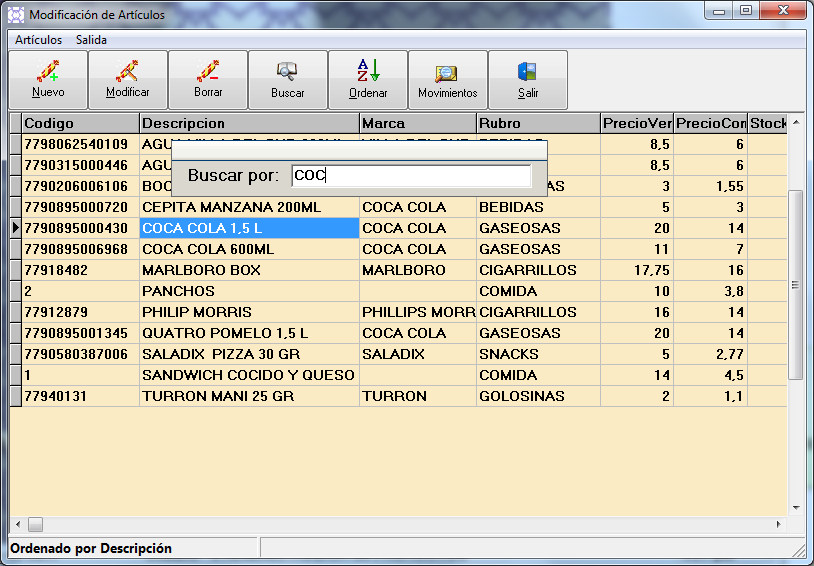
\includegraphics[scale=0.4]{gds.png}
    \caption{Ejemplo del GDS Software}
    \label{fig:enter-label}
\end{figure}

Su ventaja es la facilidad de uso con acceso rápido, menú interactivo y opciones de búsqueda rápida, además del soporte técnico en línea por problemas que puede surgir. \\

\subsubsection{Fácil Virtual Kioscos}
es un software de gestión de ventas diseñado para pequeños y medianos negocios como kioscos, maxikioscos y drugstores. Se destaca por su facilidad de uso e interfaz intuitiva, siendo ideal para quienes la usan por primera vez en su negocio. \\
Ofrece estas funcionalidades:\cite{facilvirtualSoftwarePara}
\begin{itemize}
	\item \textbf{Control total de caja}: registra ventas, compras, gastos e ingresos y egreso de dinero.
	\item \textbf{Gestión de usuarios y turnos}: cada usuario tiene su clave de acceso y se le pueden asignar permisos o privilegios específicos.
	\item \textbf{Control de stock}: permite llevar un registro detallado del inventario, alertando sobre productos con bajo stock y facilitando la realización de pedidos a proveedores.
	\item \textbf{Actualización de precios}: permite actualizar lista de precios de forma masiva, ya sea por su marca, rubro o código de producto.
	\item \textbf{Generación de informes}: ofrece diversos reportes sobre ventas, stock valorizado, ganancias, productos más vendidos, entre otros.
	\item \textbf{funciones adicionales}: incluye botones de acceso rápido, menús intuitivos, búsquedas rápidas, agenda de clientes, facturación electrónica, impresión de etiquetas de precios y códigos de barras y manejo de cuentas corrientes de clientes y proveedores.
\end{itemize}

\begin{figure}[!h]
    \centering
    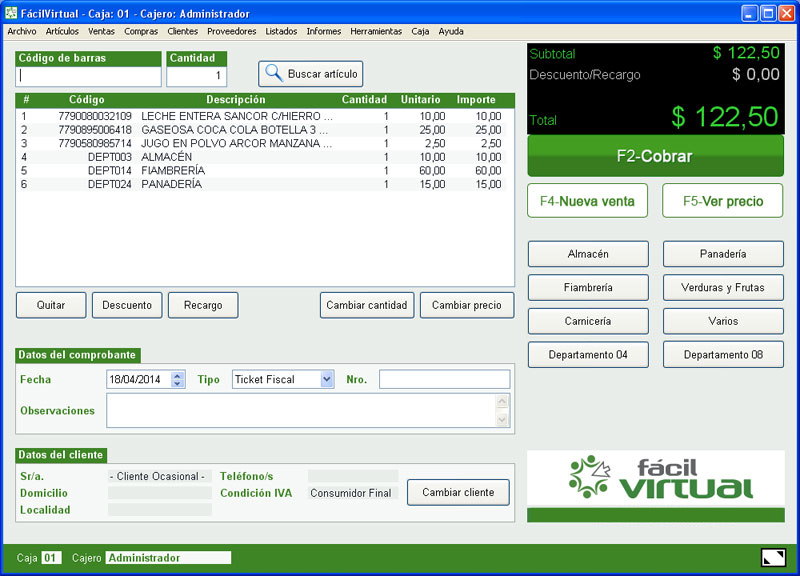
\includegraphics[scale=0.3]{facilvirtual.jpg}
    \caption{Ejemplo de Fácil Virtual Kioscos}
    \label{fig:enter-label}
\end{figure}

\subsection{¿Qué diferencia estos sistemas que ya existen, con mi proyecto?}
A diferencia de otros sistemas de gestión comercial, este proyecto fue diseñado específicamente para kioscos o comercios minoristas de bajos recursos que no disponen de computadoras ni lectores de código de barras, y que suelen manejar sus precios y ventas de forma manual.
Las principales características que lo diferencian de soluciones tradicionales son:
\begin{itemize}
	\item \textbf{Adaptabilidad a celulares}: el sistema funciona desde cualquier teléfono con cámara y navegador. Esto lo hace más accesible para negocios pequeños.
	\item \textbf{Escáner de código de barras desde la cámara}: al escanear el producto con el celular, el sistema muestra el precio exacto y actualizado, evitando errores o decisiones improvisadas al momento de la venta.
	\item \textbf{Actualización automática o manual de precios}: el sistema permite cargar boletas de proveedores, actualizar precios desde ellas, y asignar valores sugeridos para cada producto. Esto evita pérdidas por vender a precio desfasado o excesivo.
	\item \textbf{Ejecución sobre servidores LinuxONE con módulos COBOL}: a diferencias de los sistemas comunes, este proyecto se ejecuta sobre una arquitectura empresarial robusta, utilizando COBOL para procesar funciones críticas como reportes, control de stock o tareas por lotes.
	\item \textbf{interfaz intuitiva}: está diseñado para usarse sin conocimientos técnicos, permitiendo que tanto el dueño como empleados puedan operar el sistema con fluidez desde el celular.
	\item \textbf{Movilidad y acceso en tiempo real}: al estar basado en web y optimizado para dispositivos móviles, se puede consultar el stock o el historial de ventas desde cualquier lugar.
    \item \textbf{Funciones exclusivas para kioscos}: a diferencia de otros sistemas genéricos, este incluye lógica específica para:
    \begin{itemize}
        \item Control de vencimientos.
        \item Clasificación por lote y rubro.
        \item Sugerencia de promociones según productos próximos a vencer.
        \item Ubicación precisa dentro del depósito.
    \end{itemize}
\end{itemize}
Este conjunto de características convierte a esta aplicación en una solución completa, asequible y adaptada a la realidad cotidiana de los kioscos, resolviendo problemas que otros sistemas aún no contemplan.

\subsection{¿Qué es el código de barras?}\par
Es un conjunto de cifras con una estructura predeterminada, su objetivo es identificar el producto, ítem, servicio, etc. El sistema permite la individualización, origen y destino final facilitando la libre circulación de la mercadería.\cite{bibliotecaCodigoBarras} \par

\textbf{EAN:} (European Article Numbering): es un estándar internacional creado en Europa en 1977 y permite identificar productos comerciales por medio de código de barras. Opera en más de 80 países y es compatible con el sistema \textbf{UPC} (Universal Product Code), usado en America del Norte.\par
En Argentina funciona desde 1985 y los alimentos constituyen el 50\% aproximadamente de los códigos registrados.\par
Se clasifican en:
\begin{itemize}
    \item \textbf{EAN - 13:} es la versión más difundida a nivel mundial:
    \begin{itemize}
        \item Su código es de 13 cifras, (existe una versión corta de 8 posiciones que se usa cuando el espacio disponible para la impresión es pequeño).
        \item Las tres primeras posiciones que forma el prefijo EAN en Argentina es el \textbf{\textit{779}}.
        \item Las cuatro posiciones siguientes corresponden al código de la empresa. Los cinco dígitos restantes son administrados por el fabricante que identifican al producto y la decimotercera posición es una cifra de control que permite verificar si las cifras precedentes han sido correctamente leídas.\cite{dynamsoftComprehensiveGuide}
    \end{itemize}

\begin{figure}[H]
  \begin{center}
    \subfigure[EAN 8]{
        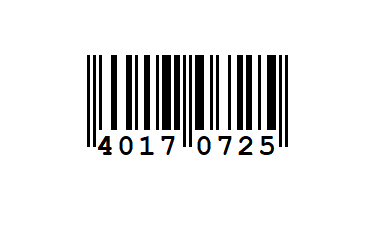
\includegraphics[scale=0.6]{EAN8.png}
        \label{Imagen-EAN8}}
    \subfigure[EAN 13 ]{
        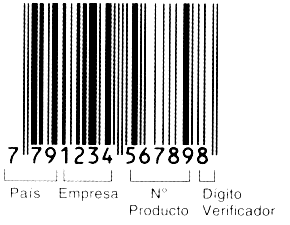
\includegraphics[scale=0.7]{EAN13.png}
        \label{Imagen-EAN13}}
    \caption{Códigos EAN}
    \label{Figuras-Codigos}
  \end{center}
\end{figure}
\end{itemize}


\subsection{Software de código de barras}
\subsubsection{Barcode for PC}
Barcode to PC es una aplicación móvil que permite a los usuarios enviar fácilmente códigos de barras a programas informáticos y automatizar tareas. Puede instalarse sin necesidad de una cuenta y funciona emulando un teclado, escribiendo códigos de barras directamente en los programas o añadiéndolos a archivos CSV. Transmite datos de forma privada a través de una red local y puede adquirir códigos de barras 1D y 2D, incluidos códigos QR.\cite{barcodetopcBarcodeWiFi}


\begin{figure}[!h]
        \centering
        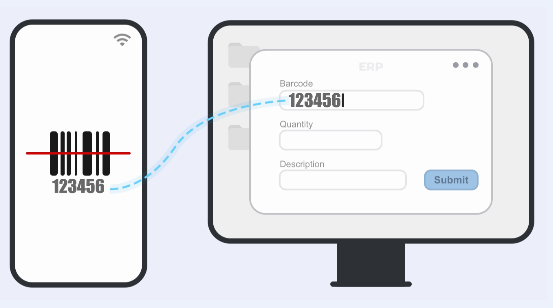
\includegraphics[width=0.5\linewidth]{barcodetoPC.png}
        \caption{Ejemplo - Barcode To PC}
        \label{fig:enter-label}
    \end{figure}

\subsubsection{QR \& Barcode Reader}
QR \& Barcode Reader es una aplicación móvil gratuita que puede escanear códigos QR y códigos de barras para obtener información adicional. Es compatible con todos los formatos, puede realizar acciones relevantes en función del código escaneado y prioriza la seguridad y el rendimiento. \\ También tiene características como linterna y zoom para escanear en diferentes entornos, la capacidad de crear y compartir códigos QR, opciones de búsqueda personalizadas y exportación CSV.\cite{googleBarcodeReader}

\begin{figure}[H]
    \centering
    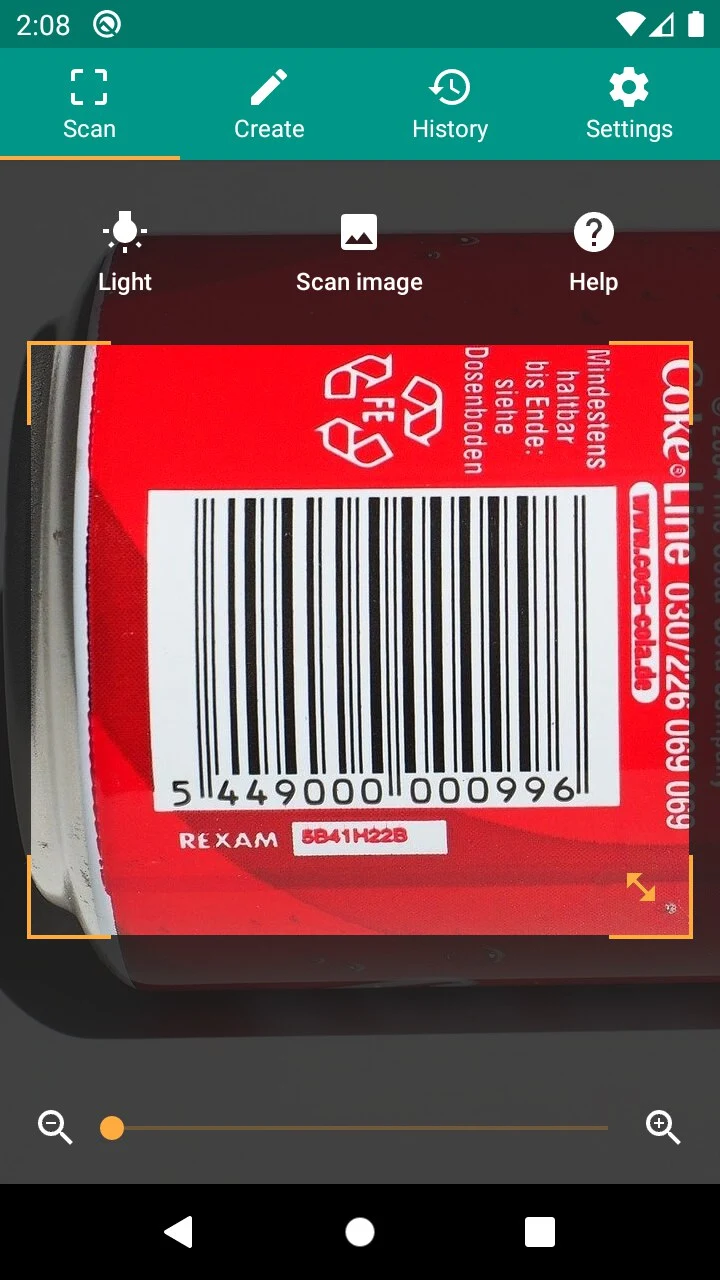
\includegraphics[width=0.3\linewidth]{QR Barcode.png}
    \caption{Ejemplo - QR \& Barcode Reader}
    \label{fig:enter-label}
\end{figure}

\subsection{Empresas que utilizan escaner de código de barras con el celular}
\subsubsection{Carrefour}
Carrefour posee una app donde tiene la opción de escanear el código de barras (de acuerdo al comercio correspondido en tu localidad), y muestra el precio del producto desde el celular, sin necesidad de estar dentro del comercio.

Esta aplicación se puede encontrar aquí: \cite{googleCarrefourArgentina} \\
Y su descripción es:\par
\textit{Entrar es muy fácil: accede con tu DNI y contraseña desde tu cuenta Mi Carrefour y podrás encontrar promociones, descuentos y muchas más ventajas.}

Además, con la App Carrefour podrás:
\begin{itemize}
    \item Acceder fácilmente a los datos de tu cuenta Mi Carrefour.
    \item Escanear los códigos de barras de los productos para corroborar su precio.
    \item Recibir notificaciones sobre promociones y descuentos.
    \item Ver las promociones semanales de Carrefour.
    \item Ver los folletos con las promociones vigentes.
    \item Ver la información de tu sucursal Carrefour más cercana.
    \item Realizar compras en carrefour.com.ar
    \item Modificar datos de tu perfil guardados en Mi Carrefour, como email, teléfono o contraseña.
\end{itemize}


\newpage
\begin{figure}[H]
  \begin{center}
    \subfigure[Pantalla principal]{
        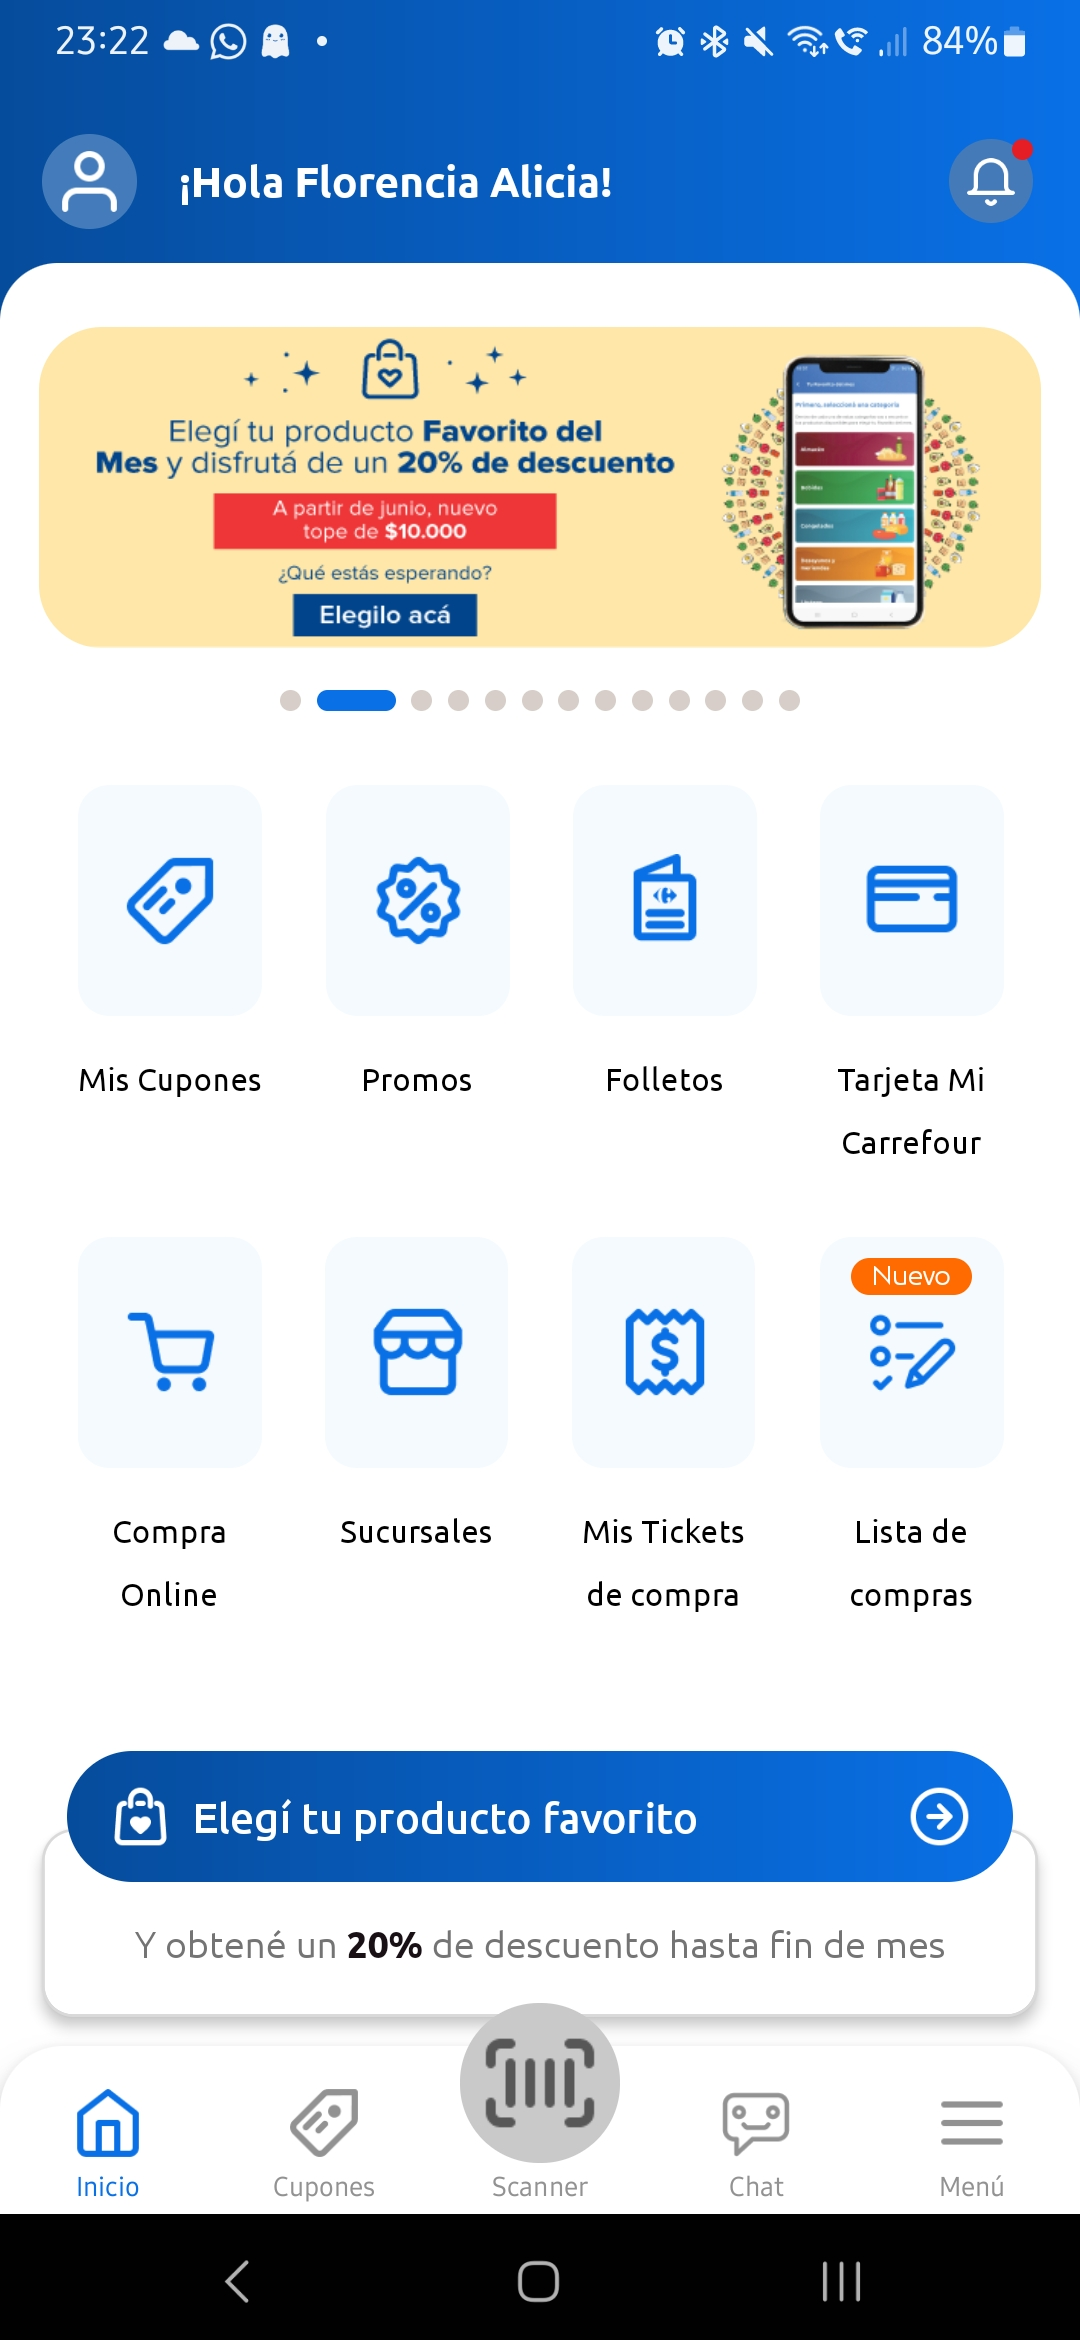
\includegraphics[scale=0.12]{Screenshot_20240624_232225_Carrefour.jpg}
        \label{Imagen-Madrid}}
    \subfigure[Escaner barcode]{
        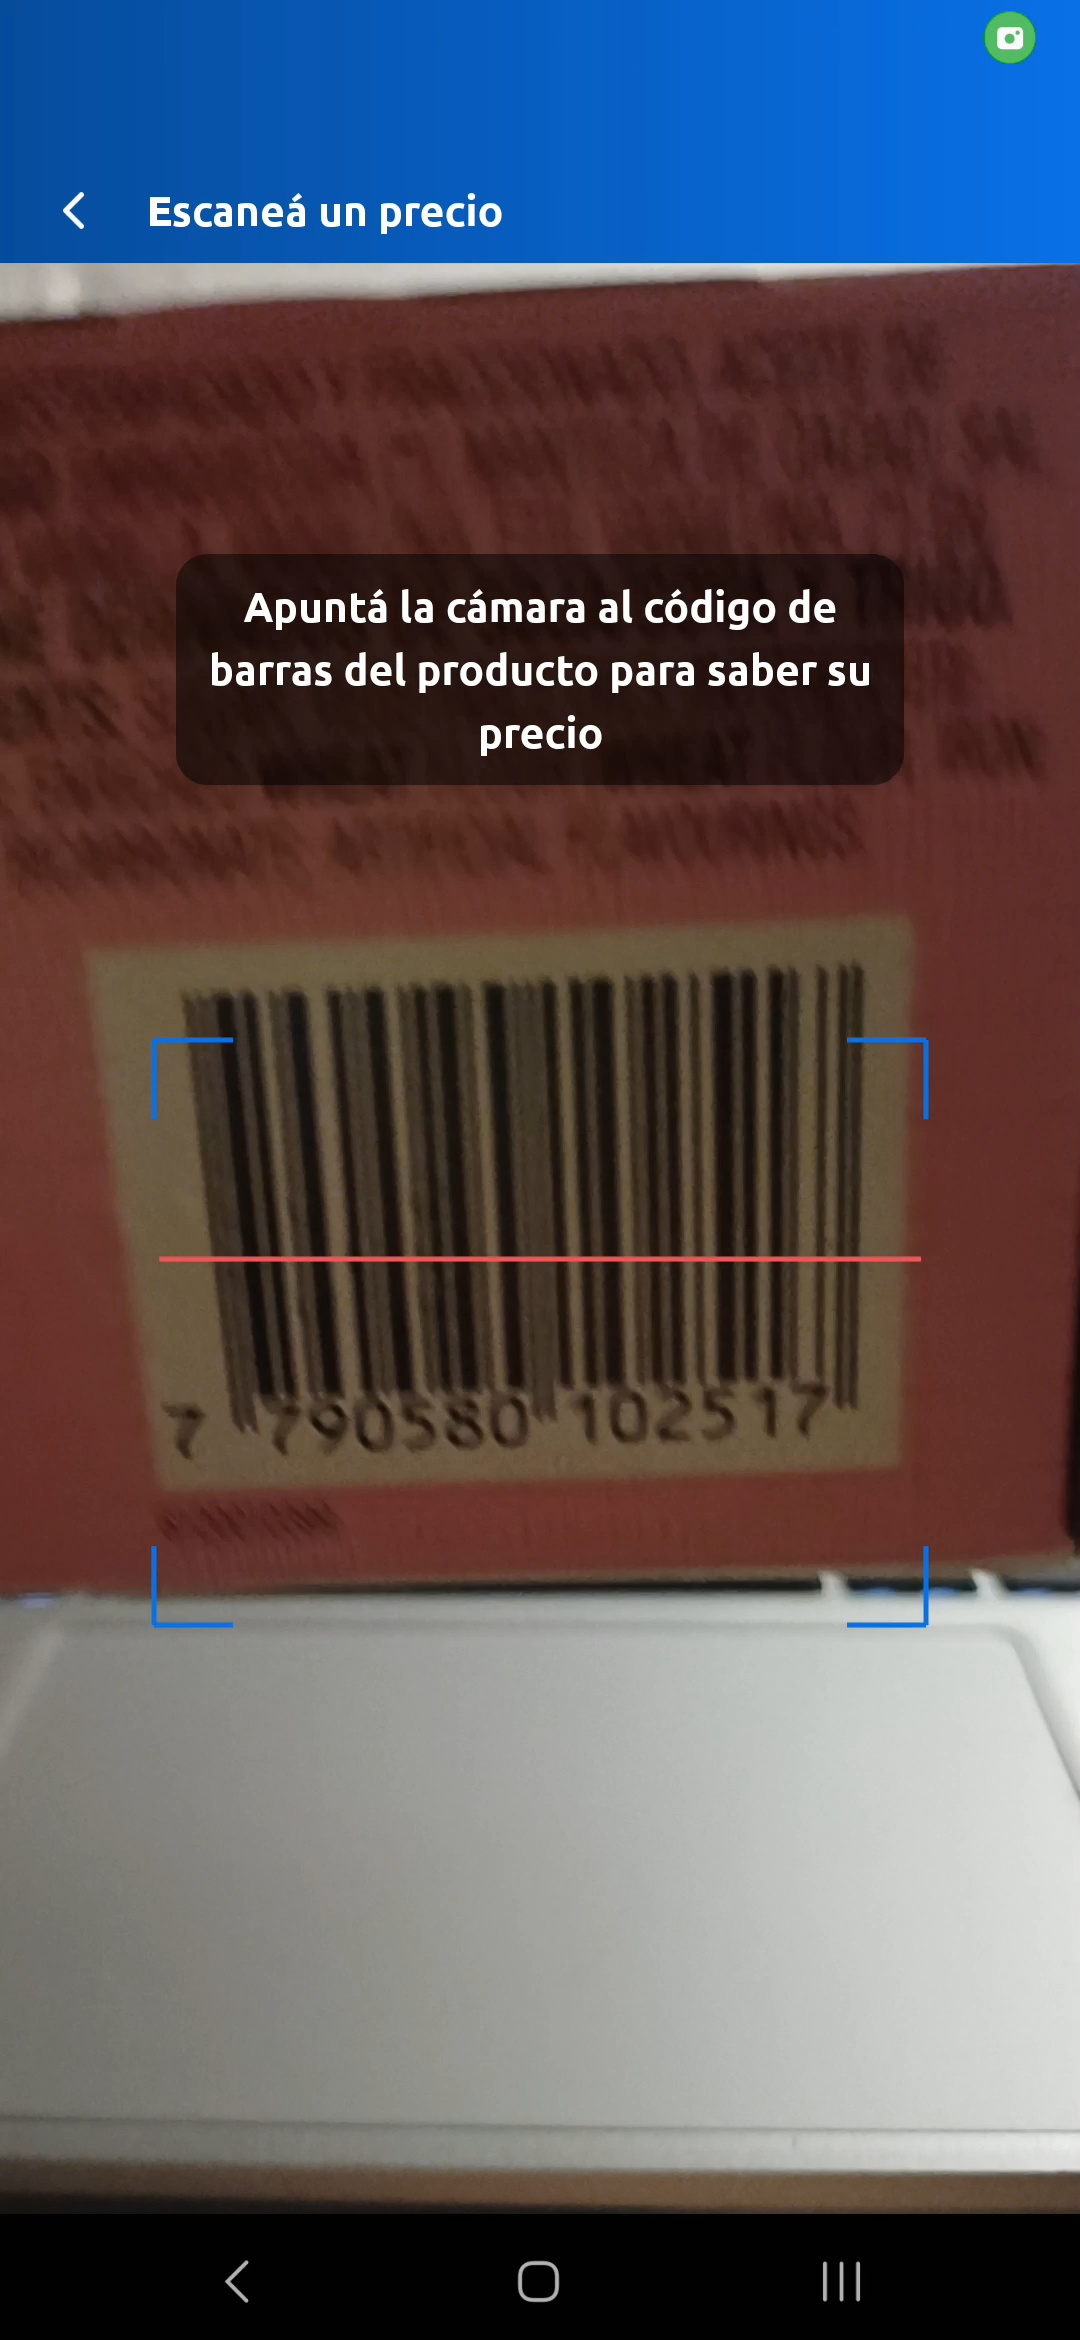
\includegraphics[scale=0.12]{Screenshot_20240624_232405_Gallery.jpg}
        \label{Imagen-Londres}}
    \subfigure[Precio del producto]{
        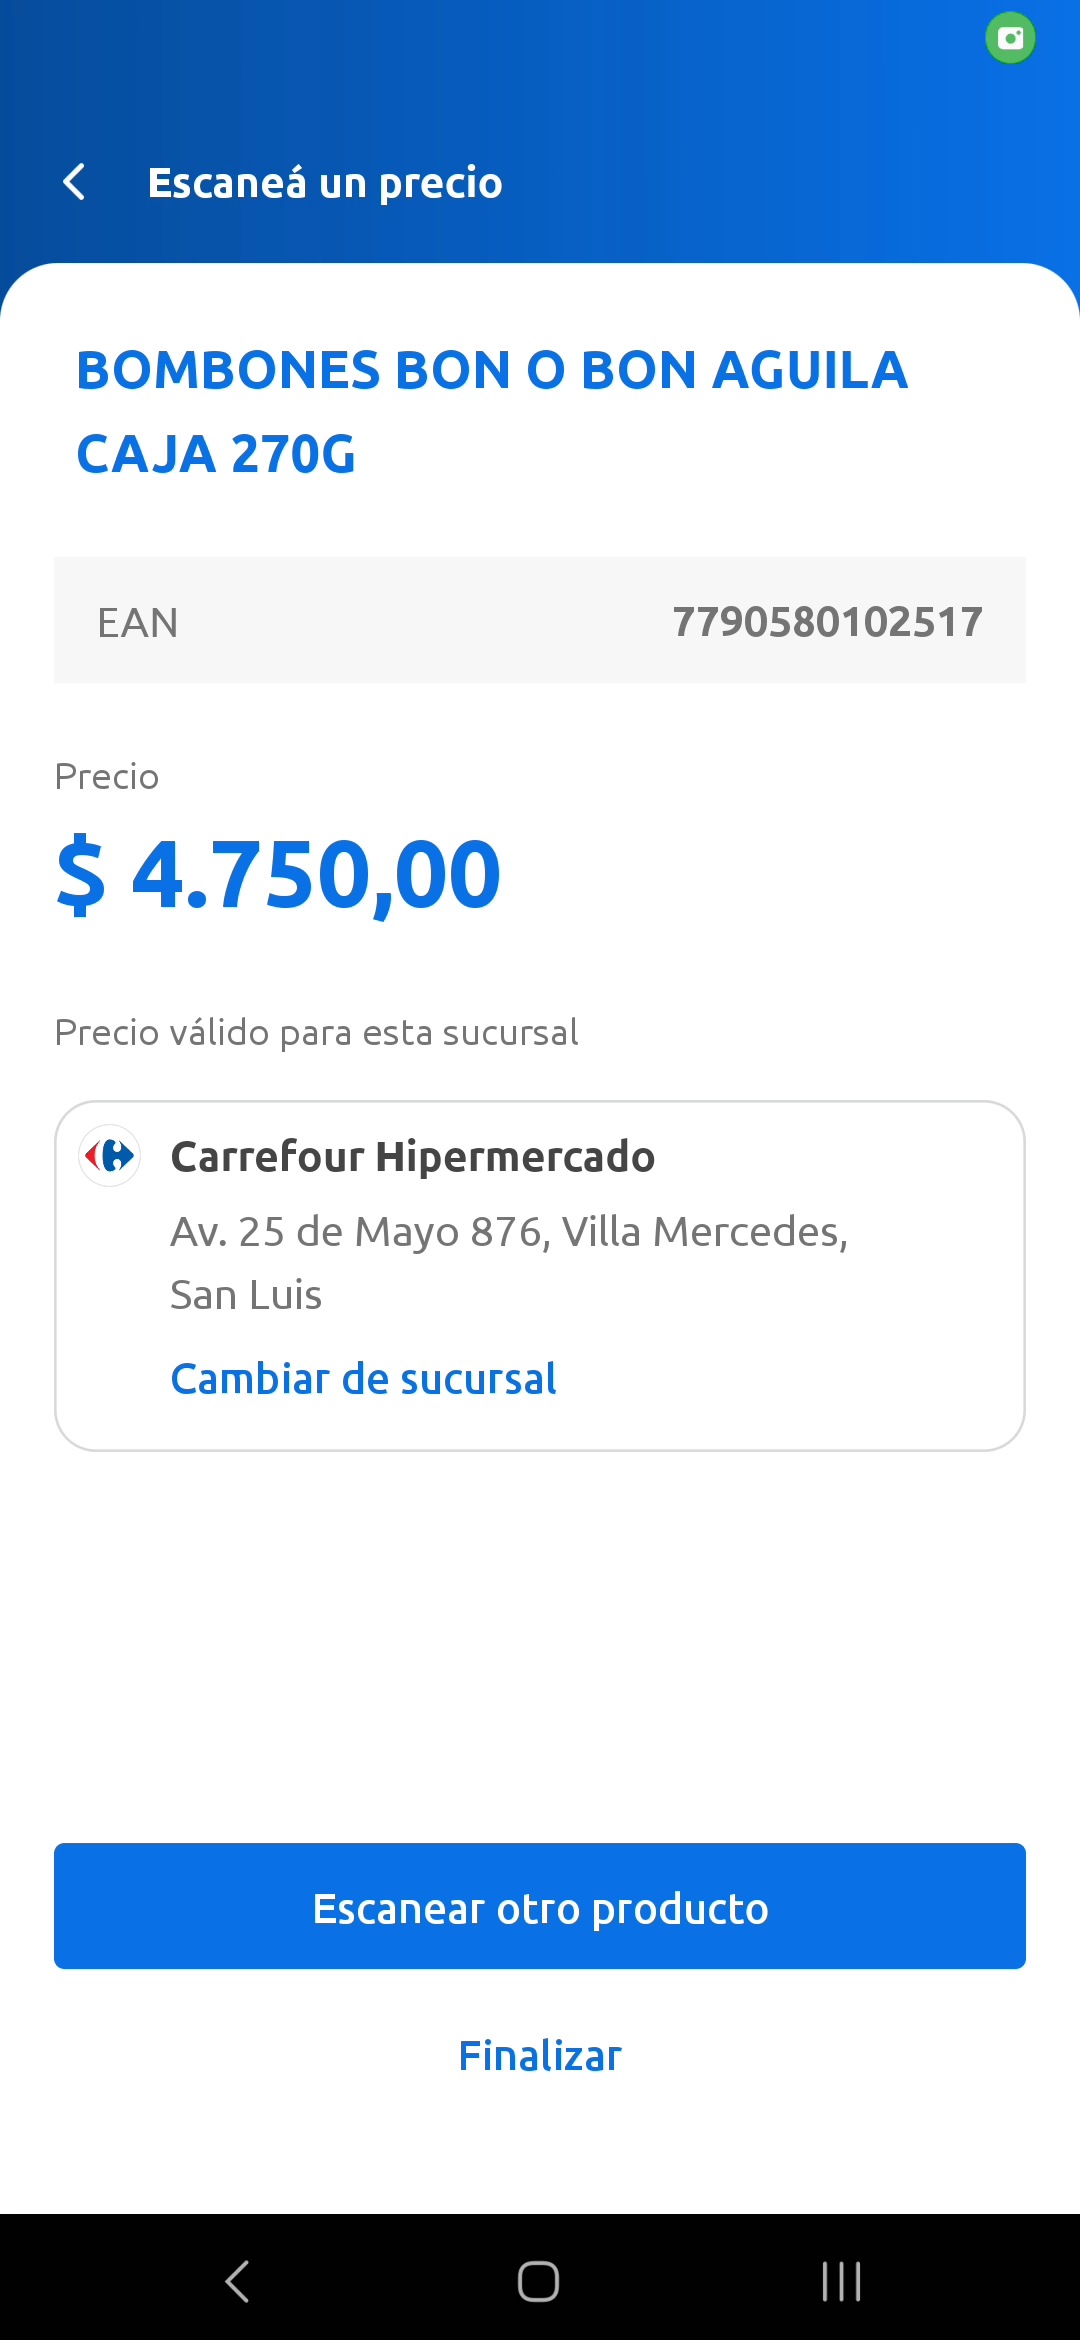
\includegraphics[scale=0.12]{Screenshot_20240624_232414_Gallery.jpg}
        \label{Imagen-Londres}}
    \caption{Carrefour APP}
    \label{Figura-Ciudades}
  \end{center}
\end{figure}


\subsection{Herramientas a utilizar}
\subsubsection{HTML}
HTML (Lenguaje de Marcas de Hipertexto, del inglés HyperText Markup Language) es el lenguaje de marcado usado para estructurar el contenido de las páginas web. En este proyecto, se emplea para construir la interfaz principal de la palicación, permitiendo la visualización de formularios, tabla de stock, campos de escaneo de productos y menús de navegación adaptados a dispositivos móviles.\cite{mozillaHTMLLenguaje}
\subsubsection{CSS}
Hojas de Estilo en Cascada (del inglés Cascading Style Sheets) o CSS es el lenguaje utilizado para definir la presentación visual del contenido HTML. Se usa para aplicar estilos, adaptar la interfaz a celulares, mejorar la experiencia del usuario y mantener una estética clara e intuitiva.\cite{mozillaCSSCascading}

\subsubsection{JavaScript}
JavaScript (JS) es un lenguaje de programación interpretado que se ejecuta en el navegador. En este sistema, se emplea principalmente para permitir el escaneo de códigos de barras desde la cámara del celular, validar formularios, manejar eventos dinámicos en la interfaz y gestionar actualizaciones de contenido en tiempo real. \cite{mozillaJavaScript}

\subsubsection{PHP}
PHP (acrónimo recursivo de PHP: Hypertext Preprocessor) es un lenguaje de propósito general ampliamente usado para desarrollo web. En este proyecto se utiliza para procesar los datos ingresados, generar alertas, cargar boletas, gestionar los registros de productos y comunicarse con la base de datos. \cite{phpPHPxBFQuxE9}

\subsubsection{COBOL}
COBOL (Common Business Oriented Language) es un lenguaje de programación histórico, especialmente diseñado para aplicacioens comerciales y financieras. En esta tesis, se implementan módulos escritos en COBOL que se ejecutan en el entorno LinuxONE, encargados de procesar tareas específicas como control de vencimientos por lote, generación de reportes y manejo eficiente de datos estructurados. \cite{ibmQuCOBOL}

\subsubsection{LinuxONE}
LinuxONE es una plataforma de mainframe de IBM diseñada para ejecutar cargas de trabajos criticas con alta disponibilidad, seguridad y escalabilidad. Se utiliza como entorno de ejecución para los procesos COBOL de este sistema, ofreciendo robustez y procesamiento empresarial en la nube. \cite{ibmLinuxONE}

\subsubsection{MYSQL / Db2}
Para el almacenamiento y gestión de datos del sistema, se usan dos tecnologías de bases de datos relacionales que cumplen funciones complementarias durante el desarrollo y la ejecución:
\begin{itemize}
    \item \textbf{MySQL}: es un sistema de gestión de base de datos (DBMS) de código abierto, ampliamente utilizado en aplicaciones web por su rapidez, estabilidad y facilidad de integración con PHP. En este proyecto, se emplea principalmente en la fase de desarrollo local, permitiendo realizar pruebas de funcionalidades, formularios y consultas SQL de manera ágil y con herramientas comunes como phpMyAdmin. \cite{mysqlMySQL}
    \item \textbf{Db2}: es un sistema de gestión de base de datos desarrollado por IBM, diseñado para manejar grandes volúmenes de información con alta seguridad y rendimiento. En este sistema, se utilizará durante la ejecución en producción dentro del entorno LinuxONE, alojando los datos principales del sistema cuando se ejecuten los procesos COBOL y se necesite una gestión más robusta de consultas, transacciones y reportes. \cite{ibmProgramacixF3nPara}.
\end{itemize}
Esta dualidad permite combinar la agilidad del desarrollo local con MySQL y la robustez del entorno mainframe con Db2, garantizando escalabilidad, seguridad y compatibilidad entre los diferentes entornos del proyecto.

\subsubsection{VS Code + Zowe CLI}
\textbf{Visual Studio Code} es el editor principal de desarrollo usado para programar módulos PHP, HTML, JS y COBOL en este proyecto.\cite{visualstudioBuildVisual} \par
\textbf{Zowe CLI }permite a los desarrolladores interactuar con el mainframe (LinuxONE) desde la línea de comandos, facilitando la carga, ejecución y prueba de programas COBOL de forma local. \cite{zoweDocs}

\subsubsection{OCR para boletas}
Para automatizar la carga de precios, se puede integrar un motor de \textbf{OCR (Reconocimiento óptico de carácteres)} que lea las boletas escaneadas o fotografiadas usando herramientas como \textbf{Tesseract OCR} o servicios en la nube como \textbf{Google API}, que permiten extraer automáticamente los datos de precios, fechas y descripciones de productos. \cite{githubGitHubTesseractocrtesseract}

\subsubsection{Libreria de escaneo de código de barras}
Para permitir el escaneo de productos directamente desde la cámara del celular, se integrará una librería JavaScript especializada en lectura de códigos de barras. Este componente forma parte esencial del sistema, ya que permite obtener el código del producto sin necesidad de hardware adicional, facilitando el acceso a la información de stock y precios en tiempo real. Una de las opciones encontradas es \textbf{QuaggaJS} ya que soporta múltiples formatos de códigos de barras y  mayor precisión en entornos variables de luz. \cite{serratusQuaggaJSAdvanced}

\newpage
\subsection{Metodologías}
En el desarrollo del sistema de gestión de kioscos, he elegido por la metodología de cascada (Waterfall) por su enfoque secuencial y estructurado, donde cada fase del proyecto se completa antes de pasar a la siguiente. 

\begin{figure}[!h]
    \centering
    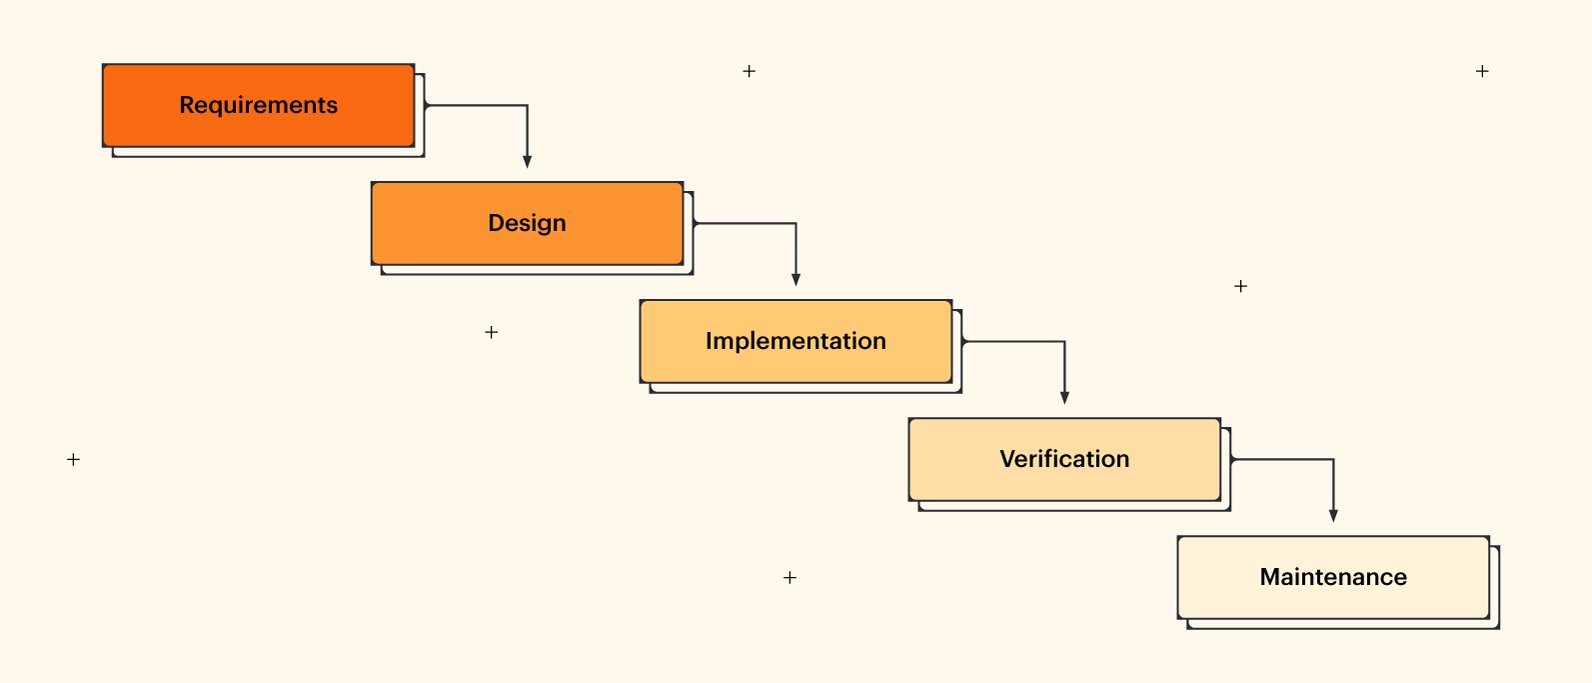
\includegraphics[scale=0.2]{WaterfallMethodologyBlogImage-2106.png}
    \caption{Metodología de Cascada - Waterfall}
    \label{fig:enter-label}
\end{figure}
\begin{enumerate}
	\item \textbf{Recolección y análisis de requisitos:} se detallan las necesidades y funcionalidad del sistema, incluyendo el control de stock por lotes y fechas, la gestión de precios, la priorización de productos próximos a vencer y la organización de la información para facilitar la toma de decisiones comerciales.
	\item \textbf{Diseño del sistema:} Se establece la arquitectura general, la estructura de la base de datos, la interfaz de usuario y la interacción del usuario con el sistema. También se diseña la lógica que permite sugerir combinaciones de productos próximos a vencer y emitir alertas para evitar pérdidas.\par
    \hspace{0.5cm} Asímismo, se establecen las estructuras de datos que serán procesadas por los \textbf{módulos COBOL}, ejecutándose en el \textbf{entorno LinuxONE} como parte del flujo principal del sistema.
	\item \textbf{Implementación}: Se desarrolla el código fuente, \textbf{tanto del front-end como back-end}, utilizando tecnologías web (PHP, HTML, CSS, JS), y se implementan los programas COBOL correspondientes, encargados de ejecutar procesos claves en el servidor LinuxONE. Ambos con \textbf{enfoque en dispositivos móviles} para facilitar el acceso desde el entorno del kiosco. \par
    \hspace{0.5cm} La comunicación entre ambos entornos se resuelve mediante integración controlada por servicios web, permitiendo que las funcionalidades se distribuyan entre \textbf{la lógica web y el procesamiento back-end}.
	\item \textbf{Pruebas y verificación}: Se testea el sistema en su conjunto, verificando el correcto funcionamiento tanto de los módulos web como de los procesos COBOL. Se evalúan casos de uso reales, consistencia de datos, respuesta ante vencimientos y ejecución en condiciones de uso normal.
	\item \textbf{Mantenimiento}: Una vez implementado, el sistema podrá recibir actualizaciones para corregir errores, optimizar el rendimiento o adaptarse a nuevas reglas comerciales, garantizando estabilidad tanto en su capa web como en los procesos mainframe.
\end{enumerate}

Esta metodología también permite generar documentación clara y exhaustiva en cada fase, lo cual es fundamental en el contexto académico de una tesis. Además brinda control sobre el ciclo de vida del sistema, asegurando que, cada etapa esté finalizada antes de avanzar, reduciendo la complejidad de gestión.

Por estas razones, se descartaron metodologías ágiles como Scrum o XP, que requieren validaciones constantes por parte de un cliente activo, o el modelo de prototipado evolutivo, ya que el sistema no se encuentra sujeto a cambios frecuentes ni desarrollo incremental.

El modelo Waterfall resulta coherente con los objetivos, el alcance funciones y el enfoque técnico del presente proyecto.



\newpage

\section{Ingeniería y Análisis de los requerimientos del software}
Para el desarrollo del sistema de gestión propuesto, se identifican los requisitos del software en función de las necesidades observadas en kioscos minoristas. Este análisis busca traducir los problemas detectados en funcionalidades concretas, considerando tanto el comportamiento esperado del sistema con sus restricciones técnicas.\par
A continuación, se detallan los distintos tipos de requisitos que guiarán el diseño e implementación del software.

\subsection{Requisitos Funcionales}
son aquellas funciones que el sistema debe realizar para cumplir su propósito:
\begin{itemize}
    \item \textbf{RF01}: registrar la entrada de productos mediante el escaneo de código de barras desde la cámara del celular.
    \item \textbf{RF02}: registrar la salida de productos al momento de la venta.
    \item \textbf{RF03}: almacenar y gestionar información por lote, incluyendo fecha de ingreso y vencimiento.
    \item \textbf{RF04}: emitir alertas cuando un producto esté próximo a vencer.
    \item \textbf{RF05}: cargar y actualizar precios automáticamente a partir de boletas mediante OCR.
    \item \textbf{RF06}: permitir la edición manual de precios, asignación de márgenes y sugerencias de precios de venta.
    \item \textbf{RF07}: visualizar en tiempo real el stock disponible por producto, lote y ubicación dentro del depósito.
    \item \textbf{RF08}: sugerir combinaciones de productos próximos a vencer para promociones u ofertas.
    \item \textbf{RF09}: generar reportes básicos sobre stock. vencimientos y movimientos.
    \item \textbf{RF10}: enviar datos estructurados al servidor LinuxONE para ser procesados por módulos COBOL.
    \item \textbf{RF11}: recibir respuestas procesadas desde COBOL y reflejar los resultados en la interfaz web (por ejemplo: informes, reordenamiento, validación de vencimientos).
\end{itemize}

\subsection{Requisitos no funcionales}
Describen características de calidad del sistema:
\begin{itemize}
    \item \textbf{RNF01}: el sistema debe ser accesible desde dispositivos móviles Android o iOS sin necesidad de instalación.
    \item \textbf{RNF02}: debe funcionar correctamente en navegadores compatibles con WebRTC y acceso a cámara.
    \item \textbf{RNF03}: el tiempo de respuesta para el escaneo de código de barras no debe exceder los 2 segundos.
    \item \textbf{RNF04}: la carga de boletas para OCR debe permitir al menos formatos .jpg, .png y .pdf.
    \item \textbf{RNF05}: la interfaz debe ser intuitiva, responsiva y apta para usuarios sin experiencia técnica.
    \item \textbf{RNF06}: la conexión entre la aplicación web y el entorno COBOL debe garantizar consistencia de datos, sin duplicados ni pérdidas.
\end{itemize}

\subsection{Restricciones}
Condiciones externas que limitan el diseño del sistema:
\begin{itemize}
    \item \textbf{R01}: el sistema será desarrollado con tecnologías web: PHP, HTML, CSS y JavaScript.
    \item \textbf{R02}: la base de datos en desarrollo será MySQL, y en producción se migrará a DB2 bajo entorno LinuxONE.
    \item \textbf{R03}: los módulos COBOL se ejecutarán en el servidor remoto provisto por IBM LinuxONE.
    \item \textbf{R04}: el uso de OCR dependerá de la calidad de imagen de la cámara del celular del usuario.
    \item \textbf{R05}: se trabajará bajo una arquitectura que separe claramente la lógica de presentación (web) y la lógica de procesos (mainframe).
\end{itemize}

\section{Diseño}
Para representar visualmente los requerimientos y el funcionamiento del sistema, se utilizarán los siguientes diagramas:

\subsection{Caso de Uso Inicial}
\begin{figure}[!h]
    \centering
    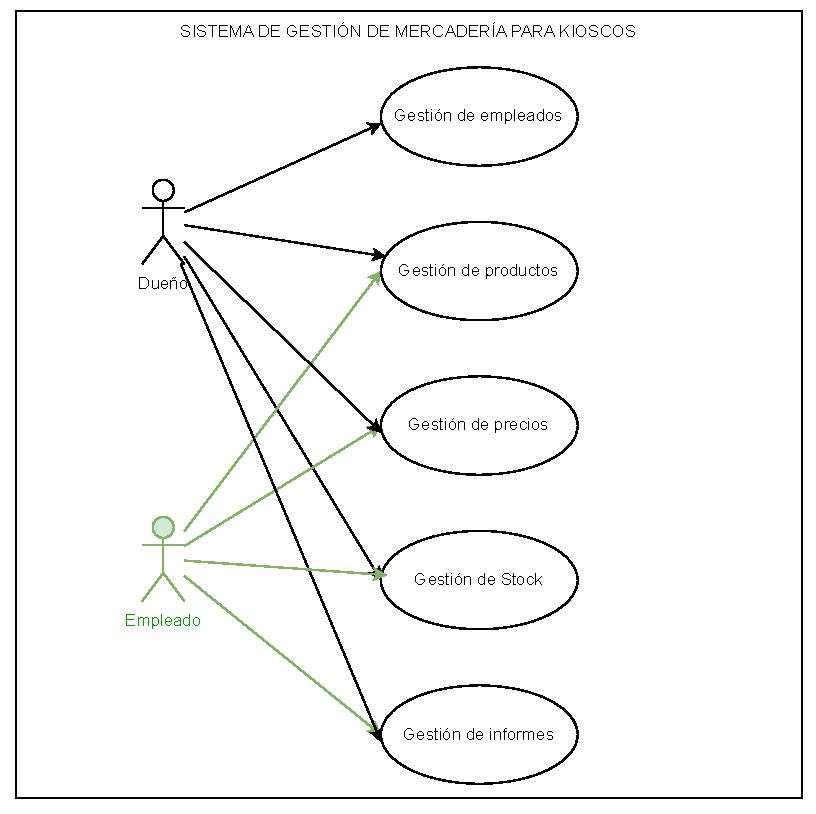
\includegraphics[scale=0.95]{casodeusoini.pdf}
    \caption{Caso de uso Inicial}
    \label{fig:enter-label}
\end{figure}

\newpage
\subsection{Caso de Uso Expandido}

\begin{figure}[!h]
    \centering
    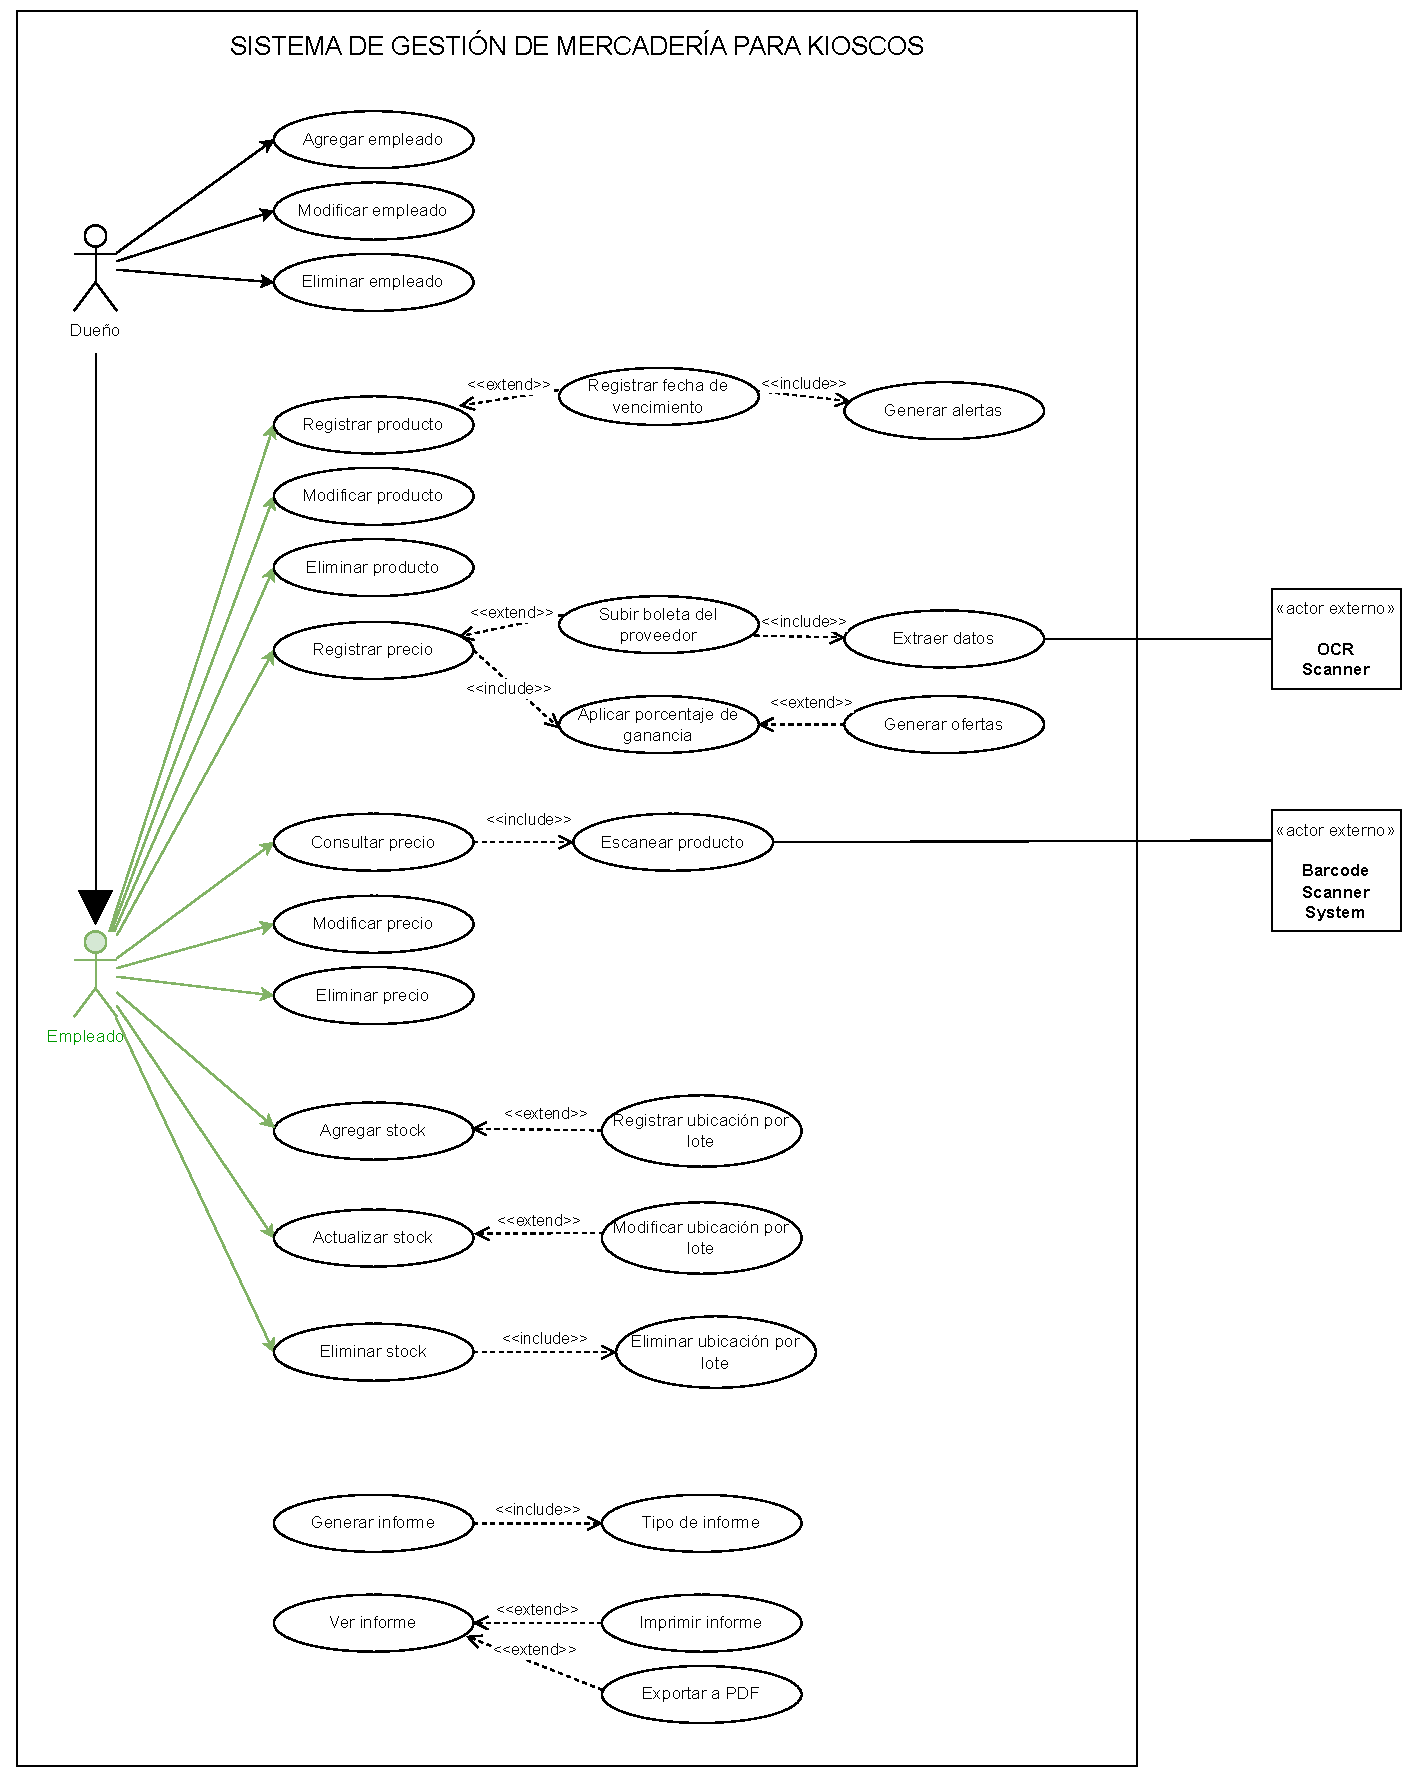
\includegraphics[scale=0.70]{casodeusoexpandido.pdf}
    \caption{Caso de uso Expandido}
    \label{fig:enter-label}
\end{figure}

\newpage
\subsection{Formularios de caso de uso expandido}
\subsubsection{Agregar empleado}
\begin{table}[!htbp] %Formulario Registro
  \centering
  \caption{Formulario caso de uso - E1a: Agregar Empleado}
    \begin{tabular}{|l|l|}
    \toprule
    \rowcolor[rgb]{ .635,  .973,  .882} \textbf{ID Caso de Uso y Nombre:} & \cellcolor[rgb]{ .867,  .922,  .969} E1a: Agregar Empleado \\
    \midrule
    \rowcolor[rgb]{ .635,  .973,  .882} \textbf{Descripción} & \cellcolor[rgb]{ .867,  .922,  .969} El dueño del kiosco agrega un nuevo empleado al sistema \\
    \midrule
    \rowcolor[rgb]{ .635,  .973,  .882} \textbf{Actores:} & \cellcolor[rgb]{ .867,  .922,  .969} Dueño (principal) \\
    \midrule
    \rowcolor[rgb]{ .635,  .973,  .882} \textbf{Prioridad} & \multicolumn{1}{p{27.07em}|}{\cellcolor[rgb]{ .867,  .922,  .969} Esencial} \\
    \midrule
    \rowcolor[rgb]{ .635,  .973,  .882} \textbf{Riesgo} & \multicolumn{1}{p{27.07em}|}{\cellcolor[rgb]{ .867,  .922,  .969} Bajo} \\
    \midrule
    \rowcolor[rgb]{ .635,  .973,  .882} \textbf{Condiciones previas:} & \multicolumn{1}{p{27.07em}|}{\cellcolor[rgb]{ .867,  .922,  .969} El dueño debe haber iniciado sesión en el sistema.} \\
    \midrule
    \rowcolor[rgb]{ .635,  .973,  .882} \textbf{Suposiciones:} & \cellcolor[rgb]{ .867,  .922,  .969} El sistema permite registrar múltiples empleados \\
    \midrule
    \rowcolor[rgb]{ .635,  .973,  .882} \textbf{Escenario Principal:} & \multicolumn{1}{p{27.07em}|}{\cellcolor[rgb]{ .867,  .922,  .969} 1. El sistema muestra campos para que el dueño complete: Nombre, Apellido, Usuario, Contraseña, Confirmar Contraseña.\newline{} 2. El dueño completa los campos.\newline{} 3. El sistema verifica los datos ingresados.\newline{} 4. El sistema registra al nuevo empleado en la base de datos y muestra un mensaje de confirmación.} \\
    \midrule
    \rowcolor[rgb]{ .635,  .973,  .882} \textbf{Escenario Alternativo:} & \multicolumn{1}{p{27.07em}|}{\cellcolor[rgb]{ .867,  .922,  .969} 3. Si los datos no son válidos, el sistema muestra mensajes de error indicando los campos incorrectos. \newline{} 4.Si el nombre de usuario ya existe, el sistema muestra un mensaje de error y solicita ingresar otro nombre de usuario. } \\
    \midrule
    \rowcolor[rgb]{ .635,  .973,  .882} \textbf{Post Condiciones:} & \cellcolor[rgb]{ .867,  .922,  .969} El empleado está registrado correctamente en el sistema. \\
    \bottomrule
    \end{tabular}%
  \label{tab:addlabel}%
\end{table}%
\newpage
\subsubsection{Registrar Producto}
\begin{table}[!htbp]
\centering
\caption{Formulario caso de uso - Registrar Producto}
\begin{tabular}{|l|p{29em}|} % Ajusta el ancho de la columna derecha según necesites
\toprule
\rowcolor[rgb]{ .635, .973, .882} \textbf{ID Caso de Uso y Nombre:} & \cellcolor[rgb]{ .867, .922, .969} Registrar Producto \\
\midrule
\rowcolor[rgb]{ .635, .973, .882} \textbf{Descripción} & \cellcolor[rgb]{ .867, .922, .969} El empleado registra un nuevo producto en el sistema, incluyendo opcionalmente la cantidad inicial en stock y la fecha de vencimiento si es perecedero. \\
\midrule
\rowcolor[rgb]{ .635, .973, .882} \textbf{Actores:} & \cellcolor[rgb]{ .867, .922, .969} Empleado (principal), sistema de escaneo de código de barras (actor externo - secundario) \\
\midrule
\rowcolor[rgb]{ .635, .973, .882} \textbf{Prioridad} & \cellcolor[rgb]{ .867, .922, .969} Esencial \\
\midrule
\rowcolor[rgb]{ .635, .973, .882} \textbf{Riesgo} & \cellcolor[rgb]{ .867, .922, .969} Alto \\
\midrule
\rowcolor[rgb]{ .635, .973, .882} \textbf{Condiciones previas:} & \cellcolor[rgb]{ .867, .922, .969} El empleado debe haber iniciado sesión en el sistema. \\
\midrule
\rowcolor[rgb]{ .635, .973, .882} \textbf{Suposiciones:} & \cellcolor[rgb]{ .867, .922, .969} El sistema está conectado al actor externo para escanear el código de barras. Se asume que el empleado podrá completar todos los campos requeridos y decidir si registrar o no el stock en el momento. \\
\midrule
\rowcolor[rgb]{ .635, .973, .882} \textbf{Escenario Principal:} & \cellcolor[rgb]{ .867, .922, .969} 1. El empleado escanea el código de barras del producto utilizando el sistema de escaneo desde la cámara del celular.\newline{} 2. El sistema muestra un formulario con los siguientes campos para completar: Nombre del producto, Categoría, Precio de compra, Porcentaje de Ganancia, Ubicación en el Depósito, Stock inicial (opcional), ¿Es Perecedero? [Sí/No].\newline{} 3. Si el producto es perecedero, el sistema muestra un campo adicional para ingresar la fecha de vencimiento.\newline{} 4. El empleado completa los campos del formulario.\newline{} 5. El sistema valida los datos ingresados.\newline{} 6. El sistema registra el nuevo producto en la base de datos y muestra un mensaje de confirmación en pantalla. \\
\midrule
\rowcolor[rgb]{ .635, .973, .882} \textbf{Escenario Alternativo:} & \cellcolor[rgb]{ .867, .922, .969} 1. Si el escaneo falla, el empleado puede ingresar el código de barras manualmente.\newline{} 2. Si los datos no son válidos, el sistema muestra mensajes de error indicando los campos incorrectos. \\
\midrule
\rowcolor[rgb]{ .635, .973, .882} \textbf{Post Condiciones:} & \cellcolor[rgb]{ .867, .922, .969} El nuevo producto está registrado en el sistema con todos sus datos. Si se trata de un producto perecedero, queda vinculado al sistema de alertas por vencimiento. Si no se ingresó stock, el sistema podrá notificarlo posteriormente. \\
\bottomrule
\end{tabular}
\label{tab:addlabel}
\end{table}
\newpage
\subsubsection{Consultar Precios}
\begin{table}[!htbp]
\centering
\caption{Formulario caso de uso - Consultar precios}
\begin{tabular}{|l|p{29em}|} 
\toprule
\rowcolor[rgb]{ .635, .973, .882} \textbf{ID Caso de Uso y Nombre:} & \cellcolor[rgb]{ .867, .922, .969} Consultar precios \\
\midrule
\rowcolor[rgb]{ .635, .973, .882} \textbf{Descripción} & \cellcolor[rgb]{ .867, .922, .969}El empleado consulta el precio de venta de un producto escaneando su código de barras mediante el sistema externo de escaneo integrado. \\
\midrule
\rowcolor[rgb]{ .635, .973, .882} \textbf{Actores:} & \cellcolor[rgb]{ .867, .922, .969} Empleado (principal), sistema de escaneo de código de barras (actor externo) \\
\midrule
\rowcolor[rgb]{ .635, .973, .882} \textbf{Prioridad} & \cellcolor[rgb]{ .867, .922, .969} Esencial \\
\midrule
\rowcolor[rgb]{ .635, .973, .882} \textbf{Riesgo} & \cellcolor[rgb]{ .867, .922, .969} Bajo \\
\midrule
\rowcolor[rgb]{ .635, .973, .882} \textbf{Condiciones previas:} & \cellcolor[rgb]{ .867, .922, .969} El empleado debe haber iniciado sesión en el sistema. \\
\midrule
\rowcolor[rgb]{ .635, .973, .882} \textbf{Suposiciones:} & \cellcolor[rgb]{ .867, .922, .969} El sistema está conectado al lector externo de código de barras (cámara del dispositivo móvil). Se asume que el producto consultado ya está registrado en la base de datos. \\
\midrule
\rowcolor[rgb]{ .635, .973, .882} \textbf{Escenario Principal:} & \cellcolor[rgb]{ .867, .922, .969} 1. El empleado escanea el código de barras del producto utilizando el lector del actor externo.\newline{} 2. El sistema busca el producto en la base de datos y muestra su precio de venta actualizado, junto con información adicional como descripción y stock. \\
\midrule
\rowcolor[rgb]{ .635, .973, .882} \textbf{Escenario Alternativo:} & \cellcolor[rgb]{ .867, .922, .969} 1. Si el escaneo falla, el empleado puede ingresar el código de barras manualmente o buscar el producto por nombre.\newline{} 2. Si el producto no se encuentra en la base de datos, el sistema muestra un mensaje de producto no registrado y sugiere iniciar el caso de uso "Registrar Producto" para completar los datos faltantes. \\
\midrule
\rowcolor[rgb]{ .635, .973, .882} \textbf{Post Condiciones:} & \cellcolor[rgb]{ .867, .922, .969} El empleado conoce eel precio de venta del producto y, si corresponde, su disponibilidad y detalles relacionados. El proceso de consulta concluye exitosamente. \\
\bottomrule
\end{tabular}
\label{tab:addlabel}
\end{table}

\newpage
\subsection{Tarjetas CRC}
\begin{figure}[!h]
    \centering
    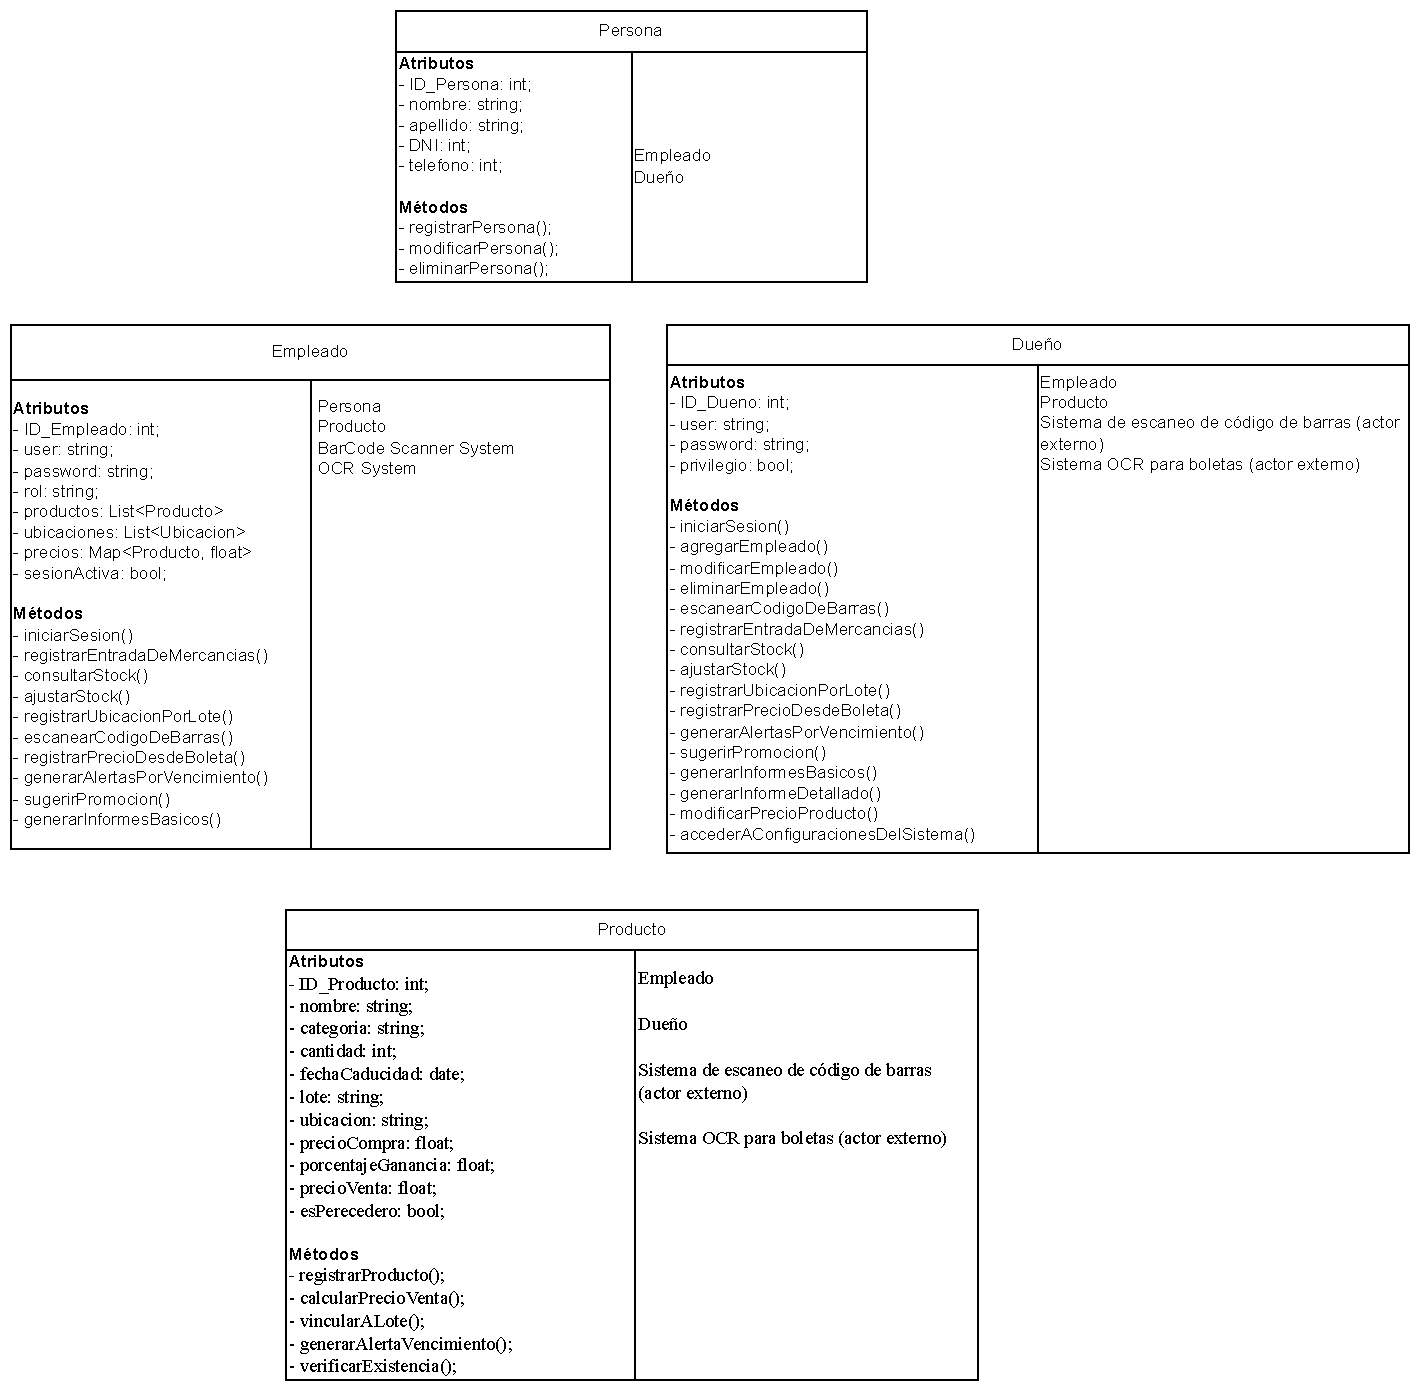
\includegraphics[scale=0.7]{CRCcards.pdf}
    \caption{Tarjetas CRC}
    \label{fig:enter-label}
\end{figure}
\newpage
\subsection{Diagrama de Actividad}
\subsubsection{Agregar Empleado}
\begin{figure}[!h]
    \centering
    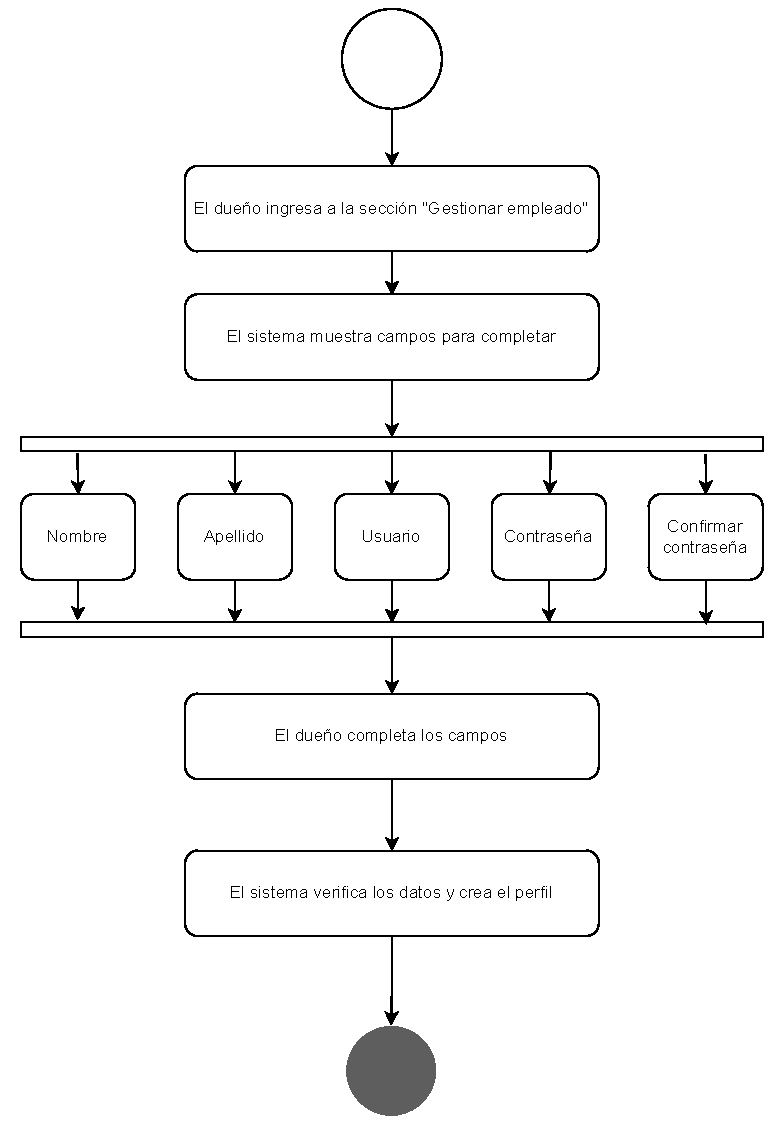
\includegraphics[scale=1]{activity1.pdf}
    \caption{Agregar Empleado}
    \label{fig:enter-label}
\end{figure}

\newpage
\subsubsection{Registrar Producto}
\begin{figure}[!h]
    \centering
    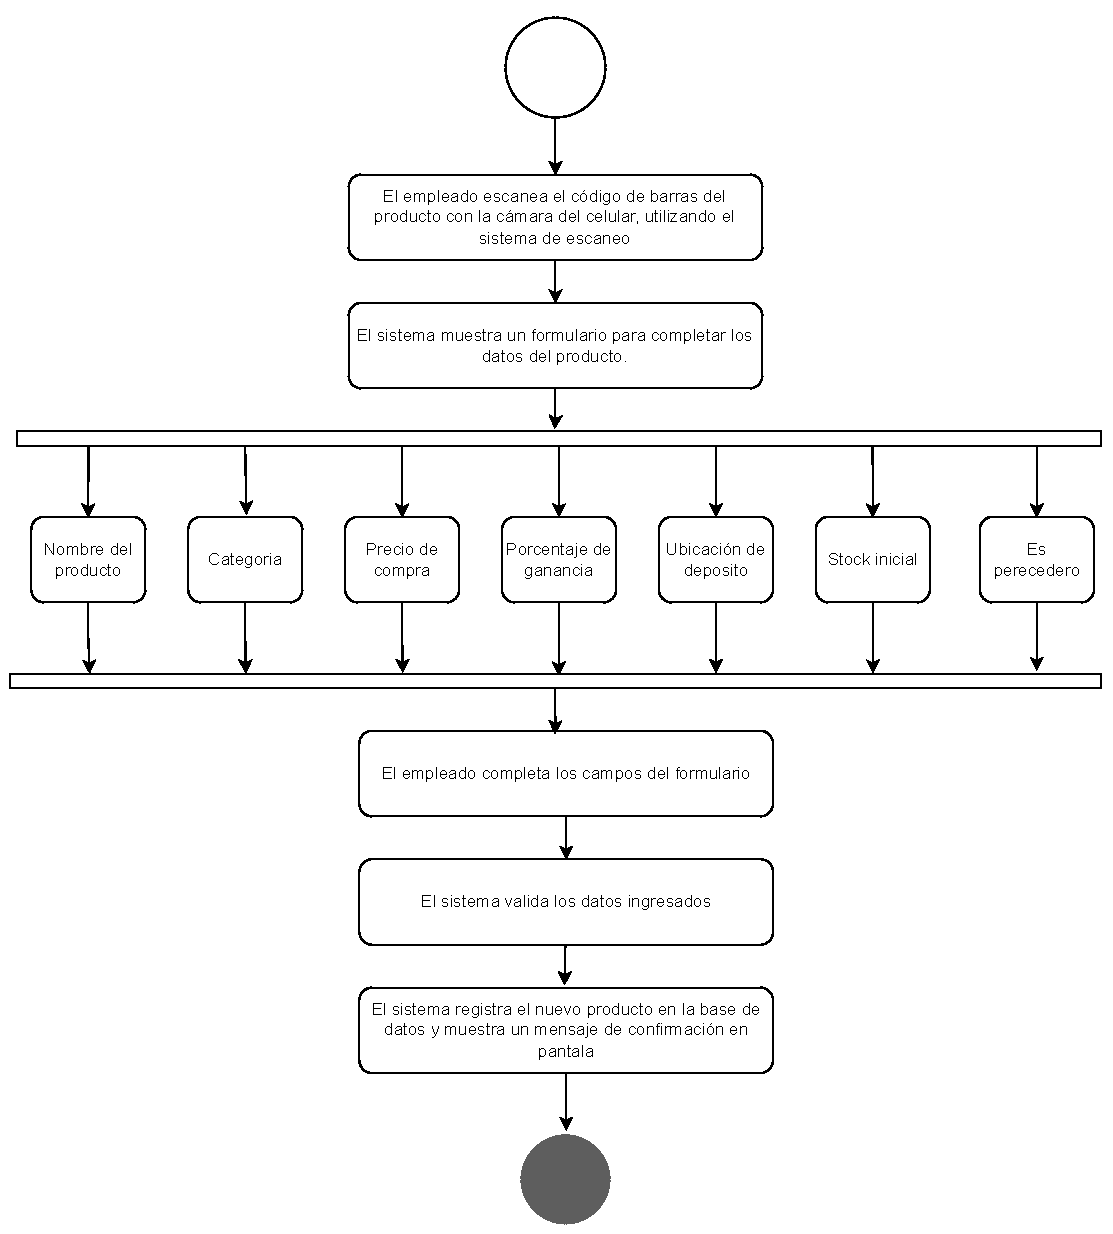
\includegraphics[scale=0.9]{activity2.pdf}
    \caption{Registrar Producto}
    \label{fig:enter-label}
\end{figure}
\newpage

\subsubsection{Consultar Precios}
\begin{figure}[!h]
    \centering
    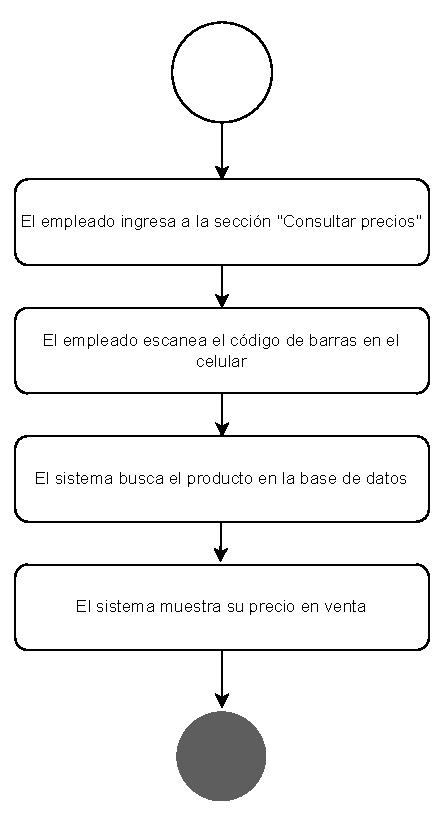
\includegraphics[scale=1.4]{activity3.pdf}
    \caption{Consultar Precios}
    \label{fig:enter-label}
\end{figure}
\newpage

\subsection{Diagrama de Secuencia}
\subsubsection{Agregar Empleado}
\begin{figure}[!h]
    \centering
    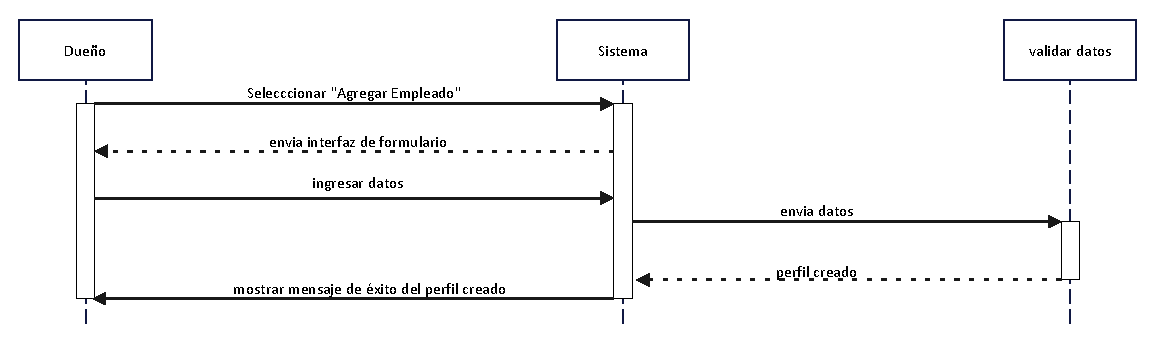
\includegraphics[scale=0.9]{sequencediagram1.pdf}
    \caption{Agregar Empleado}
    \label{fig:enter-label}
\end{figure}

\subsubsection{Registrar Producto}
\begin{figure}[!h]
    \centering
    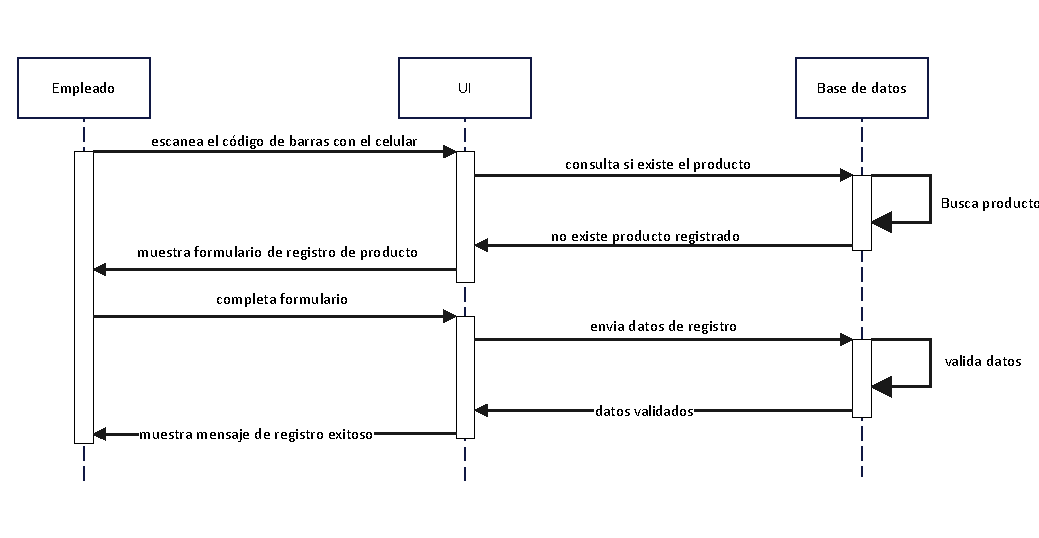
\includegraphics[scale=1]{sequencediagram2.pdf}
    \caption{Registrar Producto}
    \label{fig:enter-label}
\end{figure}

\newpage

\subsubsection{Consultar Precios}
\begin{figure}[!h]
    \centering
    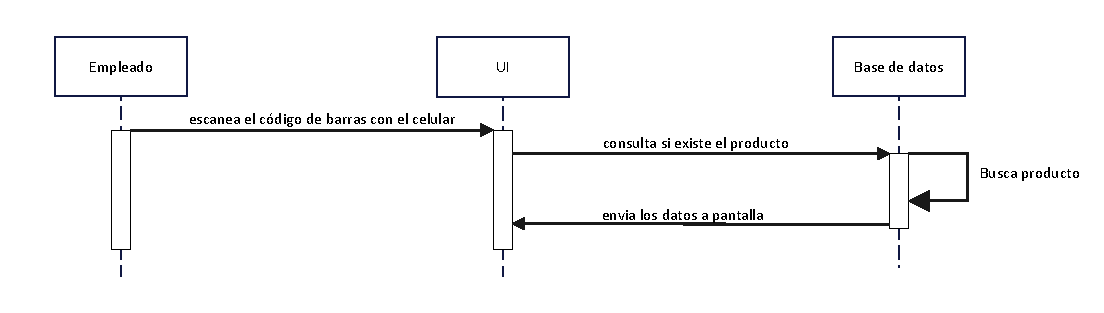
\includegraphics[scale=0.95]{sequencediagram3.pdf}
    \caption{Consultar Precios}
    \label{fig:enter-label}
\end{figure}

\newpage
\subsection{Diagrama de Base de Datos}

\begin{figure}[!h]
        \centering
        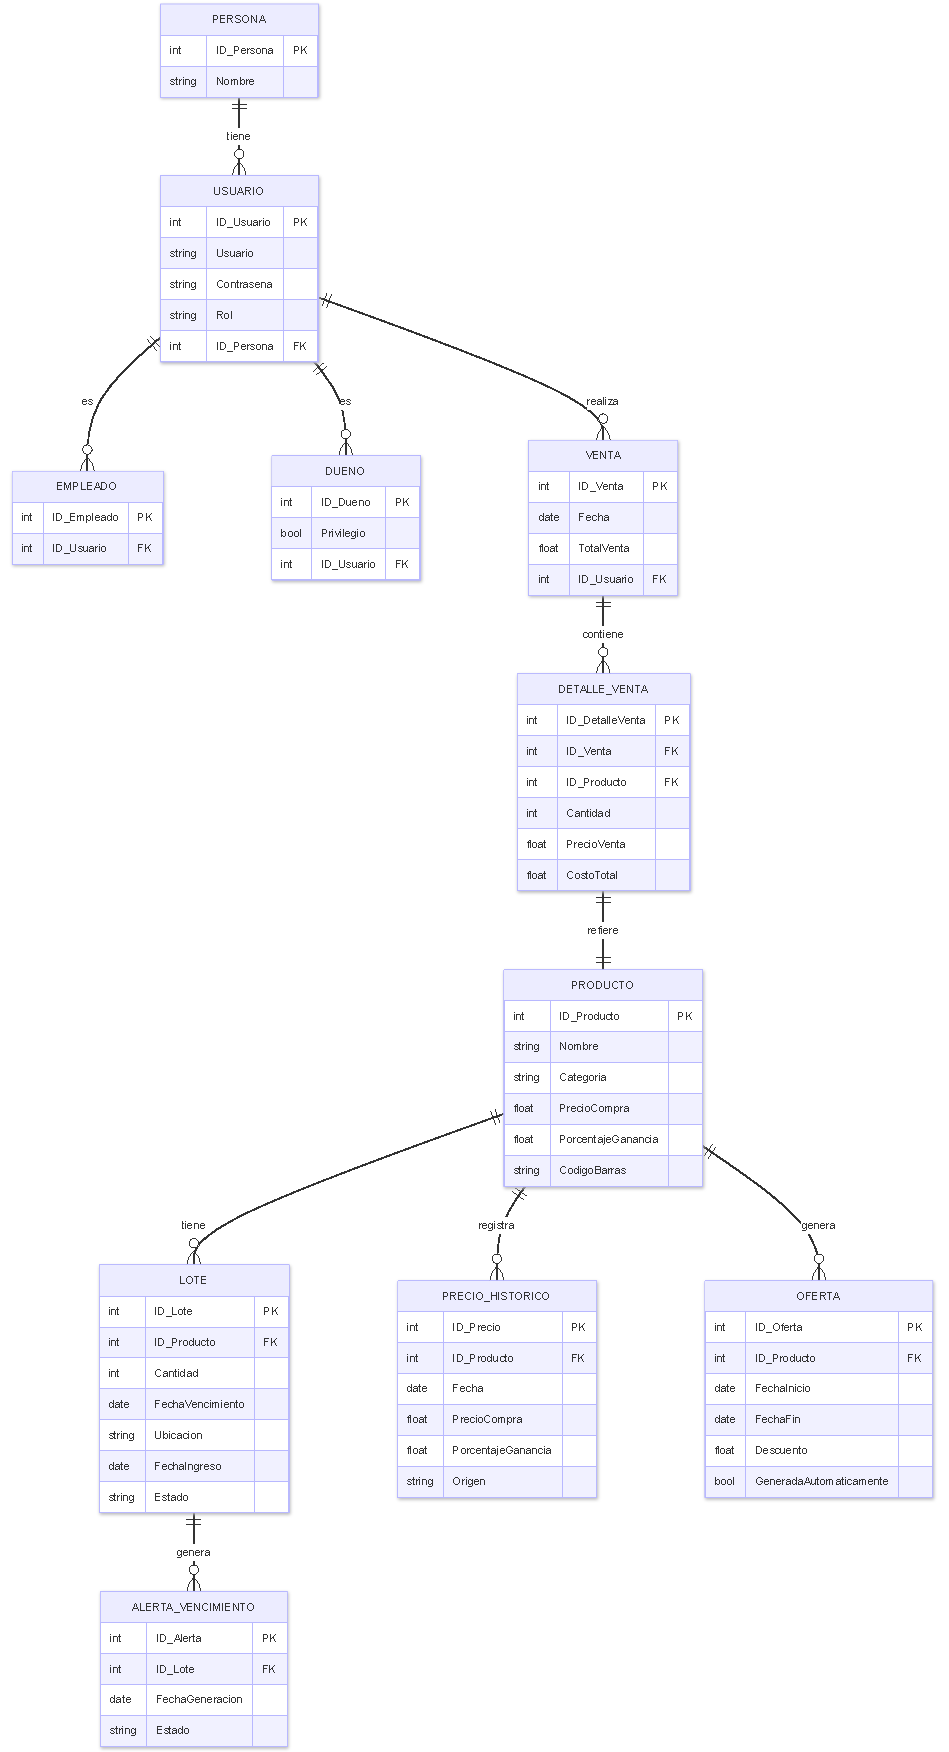
\includegraphics[width=0.73\linewidth]{diagramaBD.pdf}
        \caption{Diagrama Entidad - Relación}
        \label{fig:enter-label}
\end{figure}


\newpage






\newpage
\bibliographystyle{plain}
\bibliography{referencias}
\end{document}